
%===============PERSONAL INFORMATION===========================


%\shortauthors{Patel, Metchev, Heinze, Trollo}
%\shorttitle{Faint \WS\ Debris Disks}


%\title{}

%\author{Rahul I. Patel\altaffilmark{1}, Stanimir A. Metchev\altaffilmark{1,2}, Aren Heinze\altaffilmark{1}}
%\and
%\author{Joseph Trollo\altaffilmark{2}}
%\altaffiltext{1}{Department of Physics \& Astronomy, Stony Brook University, 100 Nicolls Road, Stony Brook, New York 11794--3800}
%\altaffiltext{2}{Department of Physics \& Astronomy, Centre for Planetary Science and Exploration, The University of Western Ontario, 1151 Richmond Street, London, Ontario, N6A 3K7, Canada}


%\begin{abstract}
%In an earlier study, we found close to a hundred previously unknown dusty disks around main sequence Hipparcos stars within 75~pc, by analyzing the distributions of their individual \WS\ colors and seeking stars with color excesses. Here, we further scrutinize the 75~pc volume of Hipparcos main-sequence stars to 1) gain sensitivity to previously undetected, fainter mid-IR excesses attributed to dusty debris disks and 2) to identify contamination of \WS\ excesses. We search for new single-color excesses by emplying an improvement over our previous method for detecting excesses, and extending this improvement to search for additional excesses by using an optimally-weighted average of shorter-wavelength \WS\ colors.   In addition, we leverage the higher resolution of the \textit{unWISE} image service to identify contaminated \WS\ excesses based on their relative astrometric offsets. 

%In total, we identify 19 previously unreported $W3$ and $W4$ single-color excesses, while only identifying two new weighted-color $W4$ excesses. The dearth of new detections from the weighted color selection is explained by the relatively large $W4$ photometric uncertainties, which dominate the errors of all $Wi-W4$ colors, from which we assert that this technique is best suited to verify single-color excesses rather than identify new ones.  Our weighted-color analysis confirms all but nine of the excesses found in our earlier work at the 99.5\% confidence level in $W4$ and 98\% confidence level in $W3$. The non-confirmations result either from the presence of marginal $W3$ excesses that diminish the significance of the $W3-W4$ excess in the weighted analysis, or from large $W1$ and $W2$ photometric errors that add mostly noise to the weighted $W4$ excess search. 

%\end{abstract}



%=======================================INTRODUCTION================================================================
\section{Introduction}
\label{sec:intro}

   Dust orbiting within several tens of AU around main sequence stars is unstable: the combination of radiative and gravitational effects eliminate it on timescales of a hundred to a few million years. The presence of such dust implies its continual generation by collisions among larger bodies (e.g., asteroids or comets) that may be  dynamically stirred by unseen planets. Identifying stars with dusty disks helps us probe the diversity of planetary system architectures and choose targets for future planet-imaging campaigns.

	Main sequence stars with debris disks are typically identified first by their infrared (IR) dust excesses: the IR fluxes at $\lambda \gtrsim$ 5\micron\ are significantly higher than would be expected from photospheric emission alone.  A debris disk can be detected by fitting a photospheric model to the shorter-wavelength (visible and near-IR) photometry, and subtracting the fitted photosphere to check for a $\gtrsim 5 \mu$m excess.  A large number of stars with IR excesses have been found this way, using data from \iras\ \citep[e.g.,][and references therein]{Moor2006, Rhee2007, Zuckerman2001}, Spitzer \citep[e.g.,][]{Su2006, Bryden2006, Trilling2008, Carpenter2009}, AKARI \citep[e.g.,][]{Fujiwara2013}, and \WS\ \citep[e.g.,][]{Cruz-SaenzdeMiera2014, McDonald2012}.
	
%	With its better sensitivity than \iras , and broad SED coverage that samples both the 3--5\micron\ stellar photosphere and potential $>5\micron$ thermal excess, \WS\ \citep{Wright2010} allows the detection of even fainter debris disks. However, the determination of an excess can be marred at different stages: either during the acquisition phase or during the post-processing phase. Filtering for contaminants introduced during either of these phases is usually half the battle.
	
	Contaminants introduced during the post-processing phase can arise from an inaccurate estimate of the photospheric emission. This usually occurs when determining the photospheric flux by photospheric modelling. The fitting approach is limited %A limitation of the photospheric model fitting approach is 
	in that it can be affected by non-simultaneity of the various photometric observations and by discrepancies among the zero-points of the various photometric systems. This problem is avoided when all of the data used to estimate the photospheric and the excess emission are measured concurrently. But for most bright stars there is no contemporaneous, precise photometry that spans a wide enough range in wavelength to produce a well-constrained photospheric fit.  Contaminants introduced during the acquisition phase, in contrast, can arise from a number of astrophysical and instrumental sources: imaging artifacts (ghosts, halos, etc.), large patches of non-uniformly distributed infrared cirrus, scattered light from the Moon, closely separated projected extra-galactic sources, projected optical companions blended into the \WS\ beam, and undiscovered Active Galactic Nuclei or Luminous Infrared Galaxies. 
	
	
	There are, however, methods to address contaminants introduced at both phases. For instance, the photospheric emission can be calibrated empirically, rather than using a model fit that will introduce additional post-processing contamination. This approach has been applied successfully to the \WS\ data: \citet{Rizzuto2012} used it to search for excesses around Sco-Cen stars based on their $W1-W3$ and $W1-W4$ colors from  the \WS\ Preliminary Release Data Release\footnote{\url{http://wise2.ipac.caltech.edu/docs/release/prelim/}} and \citet{Theissen2014} applied a similar approach to search for excesses around M dwarfs using the Sloan Digital Sky Survey Data Release 7 and the AllWISE Data Release\footnote{\url{http://wise2.ipac.caltech.edu/docs/release/allwise/}}. In \citet[][henceforth as \p14]{Patel2014}, we used the \WS\ All-Sky Survey Data Release\footnote{\url{http://wise2.ipac.caltech.edu/docs/release/allsky/}} and the \hip\ catalog \citep{Perryman1997} to determine the frequency of debris disk hosts stars within 75~pc of the Sun. To reduce contaminants accumulated from the acquisition phase, one can take advantage of survey meta-data to place filters or use crowd-sourced citizen science tools\footnote{Check out \url{http://www.diskdetective.org/}} to remove contaminated stars. %However, it always seems there is never enough meta-data for every type of contaminant, 

    In \p14, we identified stars with infrared excesses in the $W3$ and $W4$ bands by first filtering out 15 major sources of contaminants, seeking anomalously red \WS\ colors ($W1-W3, W2-W3, W1-W4$, $W2-W4$ or $W3-W4$) compared to the mean photospheric values for stars with the same Tycho $B_T - V_T$ colors, and finally removing any contaminated excess by checking their \WS\ images for background IR cirrus. We evaluated the statistical distributions of each of these \WS\ colors independently. This approach was effective, and had the advantage of not excluding stars without valid measurements in some of the \WS\ bands: for example, if $W1$ was excessively saturated, a star could still be determined to have an excess based on its $W2-W4$ or $W3-W4$ color.  However, where valid measurements exist for all \WS\ bands -- the majority of cases -- an optimally weighted combination of colors should have lower noise and potentially deliver greater sensitivity to faint excesses. 

    In this study we seek to identify high-fidelity faint IR excesses around main sequence \hip\ stars within $75$~pc by 1) using the combined weight of multiple \WS\ colors to assess a star's $W3$ or $W4$ excess, and 2) by rejecting excesses that may be contaminated from blended extragalactic sources based on the offset of their PSF centers. We motivate the selection of our sample of stars in Section~\ref{sec:sampledef}. In Section~\ref{sec:single_color_stuff}, we describe techniques for improved accuracy in the confidence threshold determination and for seeking IR excesses using weighted combinations of \WS\ colors. In Section~\ref{sec:auto_rejunwise}, we describe and apply our method for rejecting contaminated sources based on their relative positional offsets.  We use these techniques to confirm previously discovered IR excesses and to find new ones. We summarize the results of the excesses we have newly identified, verified and rejected in Section~\ref{sec:results}. In Section~\ref{sec:discussion}, we discuss our interpretation of the weighted-color excess search results and compare them to the single-color approach in \WS.


%=======================================SAMPLE DEFINITION=====================================================

        
\section{Sample Definition}
\label{sec:sampledef}

      Our sample consists of main-sequence \hip\ stars with reliable \WS\ All-Sky Catalog photometry in all four \WS\ bands. The details of the selection process are outlined in \p14. In short, we first created a parent sample of \hip\ stars within 120~pc, outside the galactic plane ($|b|>5^{\circ}$), and constrained to the $-0.17\mbox{ mag }<B_T-V_T<1.4\mbox{ mag }$ \textit{Tycho} color range. We performed additional automated screening to ensure photometric quality, consistency, and minimal contamination. We then corrected saturated photometry in the $W1$ and $W2$ bands using relations derived in \p14. Unlike in \p14, however, we included only stars that had valid photometry in $W1$, $W2$ and $W3$ bands when seeking weighted $W3$ excesses and valid photometry in all four bands when seeking weighted-$W4$ excesses.
    
  The parent (120~pc) sample provides us with a large population of stars to calibrate the photospheric \WS\ colors as a function of $B_T-V_T$. These stars are mostly within the Local Bubble \citep{Lallement2003}, and have little line-of-sight interstellar extinction ($A_V<0.05$~mag). The science sample is a 75~pc sub-sample of the parent sample, whose stars stars have accurate parallaxes. In this study, we only report and analyze detections of IR excesses from stars in the science sample.
  


\section{Single-Color and Weighted Excesses}
\label{sec:single_color_stuff}
   

%=======================================SINGLE COLOR EXCESSES================================================================

   \subsection{Improved Detection of Single-Color Excesses}
    \label{sec:improved_detection}
        
        We identify single-color \WS\ excesses based on the significance of their color excess as defined in Equation 2 of \p14
        
\begin{equation}\label{eq:old_sig}
\Sigma_{E[Wi-Wj]} = \frac{Wi-Wj-W_{ij}(B_T-V_T)}{\sigma_{ij}},
\end{equation}        
        
    \noindent where the numerator determines the $Wi-Wj$ color excess by subtracting the mean photospheric color $W_{ij}(B_T-V_T)$ at a given stellar $B_T-V_T$.  \WS\ photospheric colors do show a dependence on $B_T-V_T$ and are tabulated for the  $-0.17\mbox{ mag }<B_T-V_T<1.4\mbox{ mag }$ \citep[see published erratum;][]{Patel2014b}. Throughout the rest of this paper, the significance of a single-color excess is denoted with $\Sigma_E$.
        
    The single-color \WS\ excesses are selected by seeking stars with $\Sigma_E$ values above a certain confidence threshold. We denote the $\Sigma_E$ value at the confidence threshold CL as $\Sigma_{E_{CL}}$: CL=98\% at $W3$ and CL=99.5\% at $W4$.  In \p14, we used the excess and uncertainty distributions to calculate CL and to infer the false-discovery rate\footnote{In \p14, we incorrectly called this quantity the ``false-positive rate.''} (FDR$=1-\mbox{CL}$) at a given $\Sigma_E$ (Section~2.5 and Figure~4 of \p14). The FDR can be determined directly from the ratio of the counts of stars in the uncertainty and excess distributions. To form the uncertainty distribution for a given color, we assume that the effect of random errors on $\Sigma_E$ is symmetric with respect to zero. The various $\Sigma_E$ distributions do indeed peak close to zero (\p14), which supports this supposition. We hence assume that the negative sides of the $\Sigma_E$ distributions are representative of the negative halves of the uncertainty distributions, and so we mirror the negative $\Sigma_E$ values around the distribution peaks to obtain the full uncertainty distributions. The shapes of the combined uncertainty distributions are consistent with a Gaussian of standard deviation $\sim$~1. This indicates that our analysis is not limited by residual calibration systematics. We show an illustration of the above method in Figure~\ref{fig:ColorDist}, albeit not for the single-color excess $\Sigma_E$ metrics discussed here and in \p14, but for the weighted color \ES\ metrics introduced in Section~\ref{sec:metric}.
        
    The empirical estimate of the FDR described above and adopted in \p14 offers a straightforward method to assess the reliability of candidate excesses. However, the exact value of the $\Sigma_{E_{CL}}$ threshold tends to rely only on the one or two most-outlying stars in the (negative wing of the) $\Sigma_E$ distribution (Figure~\ref{fig:ColorDist}), and so is uncertain. In \p14 we purposefully overestimated $\Sigma_{E_{CL}}$ by the half distance to the star prior to the one that satisfied the FDR threshold. Our estimate of the $\Sigma_{E_{CL}}$ was conservative, not very accurate, and may have excluded potentially significant excesses. 
    
    Here we iterate on this approach by taking advantage of the near-Gaussian behavior of each uncertainty distribution. To circumvent the small-number sampling in the tail, we average the functional behavior by fitting a line in log-linear space to the last ten points in the rCDF of the uncertainty distribution (Figure~\ref{fig:CL_Comparison}). This continuous form of the tail of the uncertainty distribution enables a precise and more accurate estimate of the FDR. 


    %The method above---adopted in \p14---is illustrated in Figure~\ref{fig:CL_Comparison} with the reverse cumulative distribution functions (rCDFs) of the uncertainty and the excess distributions.  The FDR is simply the ratio of the two rCDFs.  Because the positive end of the uncertainty rCDF is defined by only one to two individual stars (Figure~\ref{fig:CL_Comparison}), and so is noisy, we adopted conservative estimates for $\Sigma_{E_{CL}}$ in \p14. We purposefully overestimated $\Sigma_{E_{CL}}$ by the half distance to the star prior to the star that satisfied the FDR threshold.
        
    %However, this overestimation excludes potentially significant excesses. To circumvent the small number sampling of the empirical uncertainty distribution (and improve upon our original methodology), we averaged the functional behavior in the tail by fitting a line in log-log space to the last ten points in the rCDF of the uncertainty distribution. This allows us to evaluate a continuous uncertainty distribution and provides us with a precise and more accurate estimate of the FDR. 
        
    We used the improved confidence threshold determination procedure to search for additional single-color excesses using the same set of stars and colors ($W1-W4$, $W2-W4$, $W3-W4$, $W1-W3$ and $W2-W3$) as in \p14. $W3$ and $W4$ excesses were identified at the 98\% and 99.5\% confidence levels, respectively. In addition to the excesses already identified in \p14, we found 39 additional single-color excess candidates. After inspecting and removing stars that seemed to be contaminated by background cirrus emission, we were left with 27 single-color excess candidates, 19 of which do not have IR excess detections reported in the literature. Of these 19, 18 are newly detected single-color excesses at $W4$, and one has a significant single-color excess only at $W3$, with a marginal excess at $W4$. The excess detection statistics are summarized in Table~\ref{tab:color_analysis_summary_single}. The newly detected excesses and their significances are listed individually in Table~\ref{tab:excessstats}.
        
%=======================================WEIGHTED COLOR EXCESSES================================================================
    \subsection{Defining A New Weighted IR Excess Metric}
        \label{sec:metric}
     
        In \p14 and Section~\ref{sec:improved_detection}, we identified debris disk-host candidates by selecting stars with individual anomalously red \WS\ $Wi-Wj$ colors, where $i=1,2,3$, $j=3,4$, and $i<j$. However, it may be possible to attain more reliable excess detections at $Wj$ by combining all relevant $Wi-Wj$ colors. Herein we define this new ``weighted-excess'' $Wj$ metric.
        
        As in Equation~\ref{eq:old_sig}, we first remove the contribution from the photospheric emission. Thus the single-color excess is: 

\begin{equation}\label{eq:excess_1}
        E[Wi-Wj] = Wi-Wj-W_{ij}(B_T-V_T). 
\end{equation}

\noindent Since we want to use the strength of all possible \WS\ color combinations for band $Wj$, we constructed the weighted average of the color excesses as

\begin{equation}\label{eq:wtavgExcess}
        \overline{E[Wj]} = \frac{1}{A} \sum\limits_{i=1}^{j-1} \frac{E[Wi-Wj]}{{\sigma_{Wi}}^2},
\end{equation}

\noindent where $\sigma_{Wi}$ is the photometric uncertainity of $Wi$ and $j \in [3,4]$.  Here, $A=\sum\limits_{i=1}^{j-1} \frac{1}{\sigma_{i}^2}$ is a normalization constant. Our definition for the significance $\left(\Sigma_{\overline{E[Wj]}}\right)$ of the weighted-excess at $Wj$ is the ratio of the weighted average of all color excesses (Equation~\ref{eq:wtavgExcess}) to the uncertainty in the weighted average ($\sigma_{\overline{E[Wj]}}$):

\begin{eqnarray}\label{eq:combined_significance}
    \Sigma_{\overline{E[Wj]}} &=& \overline{E[Wj]}/\sigma_{\overline{E[Wj]}}\\
            &=& \frac{\frac{1}{A}\sum\limits_{i=1}^{j-1}\frac{E[Wi-Wj]}{\sigma_i^2}}{\sqrt{\sigma_j^2 + 1/A}} . 
\end{eqnarray}

\noindent The full derivation of this metric can be found in Appendix~\ref{sec:appendix}. We use \ES\ through the rest of the paper as shorthand for the significance of the weighted excess for either $W3$ or $W4$, as appropriate, and $\Sigma_{E}$ as shorthand for the significance of the single-color excess when the discussion does not refer to any specific color.


    \subsection{Weighted-Color Excesses}
    \label{sec:weighted_excesses_results}
    
    We extend the same procedure used to identify stars with single-color excesses in Section~\ref{sec:improved_detection} to search for optimally weighted excesses in $W3$ or $W4$ using Equation~\ref{eq:combined_significance}. When discussing weighted excesses, we denote the confidence threshold as $\Sigma_{\overline{E_{CL}}}$. In Figure~\ref{fig:ColorDist}, we plot the \ES\ distributions as solid red histograms for both $W3$ and $W4$. The positive wings of the uncertainty distributions, defined analogously to those for the single-color uncertainty distributions, are shown as dashed blue histograms. The $\Sigma_{\overline{E_{CL}}}$ threshold is shown as the vertical dotted green line. We claim that a star has a significant weighted excess if its \ES\ $\geq \Sigma_{\overline{E_{CL}}}$.
    
    We identify 6 stars with 98\% significant weighted-$W3$ excesses within 75~pc of the Sun, among which we expect $2\% \times 6 = 0.12$ to be false positives. We identify 187 stars with 99.5\% significant weighted-$W4$ excesses within 75~pc of the Sun, among which we expect $0.5\% \times 187 = 0.94$ to be false positives. However, these FDRs do not account for spurious excesses caused by contamination from IR cirrus or unresolved binary companions. Hence, we checked the four-band \WS\ images for this type of contamination for all of our detections. We removed 12 of the 187 weighted-$W4$ excess sources that were deemed to be contaminated. Eleven of these 12 have single-color excess detections, which we rejected as debris disk candidates in \p14.  The other two, HIP~83221 and HIP~111136, are new false $W4$ excesses whose \WS\ images show visible line-of-sight IR cirrus contamination and are hence rejected as excesses. All 12 rejected sources are listed in Table~\ref{tab:rejects}. We were then left with 175 weighted-$W4$ excess stars. None of our weighted-$W3$ excesses seem to be contaminated based on their \WS\ images. A summary of these detections can be found in Tables~\ref{tab:color_analysis_summary_single} and \ref{tab:excessstats}.
    
\section{Automated Rejection of Contaminated Stars Using Reprocessed WISE Images}\label{sec:auto_rejunwise}

    Although improved compared to IRAS, the resolution of \WS\ is low enough to be susceptible to contamination by astrophysical sources. Stars contaminated from unresolved blended objects with non-zero colors (i.e., point-source contaminants) will adversely affect \WS's photometric and spatial properties. Stars may also be contaminated by non-uniformly distributed IR cirrus or emission from the wings of a nearby bright source (i.e., contamination from extended source emission). Both types of contaminants may manifest themselves by changing the relative position of the star between the $W3$ and $W4$ bands. To determine if any of our excesses are contaminated, we looked for significant positional centroid offsets between the $W3$ and $W4$ bands for our stars. 
    
    \subsection{unWISE Images}\label{sec:centroid_calc}
    
    Instead of using the All-Sky Atlas images, we used the higher angular resolution \textit{unWISE}\footnote{\url{http://unwise.me}} image service \citep{Lang2014}. Images from the All-Sky and AllWISE catalog were created by stacking individual exposures and then convolving each stack with a model of the detector's point-spread function (PSF). By not including this last step to create the \textit{unWISE} images, \citet{Lang2014} preserves the nominal resolution of the original stacked images. Hence, the \textit{unWISE} PSF is a factor of $\sqrt{2}$ narrower than for the All-Sky Catalog images (6\arcsec\ for $W1$, $W2$, and $W3$ and 12\arcsec\ for $W4$). We downloaded 60\arcsec\ $\times$ 60\arcsec\ (1\arcmin $\times$ 1\arcmin) $W3$ and $W4$ images from the \textit{unWISE} website for all of our excess stars, each centered around the stellar coordinates at the mean \WS\ observational epoch. We also downloaded images for 16927 Hipparcos stars within 120~pc. These stars are the union of all the stars that comprised the parent samples for the five different color excess searches in \p14: $W1-W3$, $W2-W3$, $W1-W4$, $W2-W4$, and $W3-W4$. This amalgamated sample will be used as a statistical basis for determining significant outliers amongst our excesses based on their relative positional offsets. 
    
    We hypothesized that point-source contaminants can be identified through large relative positional offsets between the centroids of the $W3-$ and $W4-$ band \textit{unWISE} images. Thus, for all our stars, we extracted centroid positions for our $W3$ and $W4$ images ($\vec{r}_{_{W3}}$ and $\vec{r}_{_{W4}}$ respectively). $\vec{r}_{_{W3}}$ and $\vec{r}_{_{W4}}$ were calculated using Gaussian centroiding in a 3.06~pixel radius aperture using a Gaussian of $\sigma=1.02$~pixels. This value of $\sigma$ was chosen to yield a full width at half maximum (FWHM) of 2.4~pixels, thus matching the FWHM of the \WS\ images. We also hypothesized that extended source contaminants could be identified by comparing the $W4$ centroid calculated in an $r=3.06$~pixel aperture to a $W4$ centroid calculated in a wider $r=10$ pixel aperture.  The $W4$ centroid calculated using the wide aperture radius is denoted as $\vec{r}_{_{W4},_{wide}}$. The 10 pixel radius ($\sim$25\arcsec\ ) extends to roughly twice the FWHM of the $W4$ PSF, and incorporates the radial distance of the first Airy ring. This ensures that any flux from the wings of the PSF from a nearby source will be flagged as a contamination source. 
    
    
    \subsection{Calculating Rejection Thresholds}\label{sec:unwise_rejectmethod}
 
    
    The density clouds in Figures~\ref{fig:w3w4_snrvsep} and \ref{fig:w4w4_snrvsep} show the distributions of our stars' $W4$ SNRs as a function of the $W3$ to $W4$ relative centroid offsets ($\Delta r_{W3,W4} = \left|\vec{r}_{_{W3}} - \vec{r}_{_{W4}}\right|$) as well as a function of the $W4$ to wide-$W4$ centroid offsets ($\Delta r_{W4} = \left|\vec{r}_{_{W4}} - \vec{r}_{_{W4},_{wide}}\right|$). Contaminated stars will therefore be located at larger separations compared to the majority of the (uncontaminated) stars that populate the cores of the centroid offset distributions. 
    
    We aimed to find the separation beyond which stars can be considered contaminated. Since the spread of separations varies as a function of $W4$~SNR, we performed this analysis using logarithmically spaced bins in $W4$~SNR space. Assuming that the core of the $j^{th}$ SNR bin was normally distributed, we defined the maximum allowed separation in each bin $\Delta r_{j,max}$ such that 
    
    \begin{equation}\label{eq:max_sep}
    \Delta r_{j,max} = 3\sigma_j,
    \end{equation}
    
    \noindent where $\sigma_j$ is the standard deviation of the azimuthally symmetric 2D Gaussian $\Delta x$ vs. $\Delta y$ distribution in the $j^{th}$ $W4$ SNR bin (i.e., $\sigma_j = \sigma_{\Delta x} = \sigma_{\Delta y}$). To calculate $\sigma_j$, we assumed first that the $\Delta x$ and $\Delta y$ offsets (used to create $\Delta r$) are distributed as a circular 2-dimensional Gaussian. A fit to this multi-variate Gaussian would then yield $\sigma_j$. 
    
    %such that more than twice the expected number of outliers exist beyond $\Delta r_{j,max}$
    
    %\begin{equation}\label{eq:max_sep}
    %\frac{1 - \Phi^j\left(\Delta r_{j,max}; \sigma \right)}{1-\Phi^j_E\left(\Delta r_{j,max}\right)} = \frac{1}{2}. 
    %\end{equation}


  %\noindent Here, $\Phi^j\left(\Delta r; \sigma \right)$ denotes the cumulative distribution function (CDF) of an optimal Gaussian distribution that represents the core of the distribution in the $j^{th}$ SNR bin. $\Phi^j_E\left(\Delta r\right)$ is the discrete the empirical CDF, calculated from the cumulative sum of the data. To calculate $\Phi^j\left(\Delta r\right)$, we assumed first that the $\Delta x$ and $\Delta y$ offsets (used to create $\Delta r$) are distributed as a circular 2-dimensional Gaussian. $\Phi^j\left(\Delta r\right)$ could then be calculated by fitting a circular 2-D Gaussian and integrating radially. 
  
  According to the WISE Explanatory Supplement, however, the major and minor axes of the WISE PSF FWHM differ (6.1\arcsec\ and 5.6\arcsec\ for the major and minor axes in $W1$, 6.8\arcsec\ and 6.1\arcsec\ for $W2$, 7.4\arcsec\ and 6.1\arcsec\ for $W3$, and 12.0\arcsec\ and 11.7\arcsec\ for $W4$). Therefore, the morphologies of the 2-D $\Delta x$ vs. $\Delta y$ distributions are also elliptical. To simplify calculations, we opted to circularize the elliptically distributed data. %Figure~\ref{fig:unwise_transform} illustrates this process. 
  Stated simply, we circularized the distributions by scaling the major axis by the ratio of the standard deviations along the minor to major-axes of the $\Delta x$ vs. $\Delta y$ distributions. % To describe it step-by-step, we:
  
  %\begin{enumerate}
  %\item Identified the position angle $\theta$ by performing a principal component analysis on a 2$\sigma$-clipped subset of the distribution
  % \item de-rotated the distribution by $\theta$.
  %\item calculated $\sigma_x$ and $\sigma_y$ of the de-rotated data. These represent the magnitude of the major and minor-axes respectively.
  %\item scaled the data by $\sigma_y/\sigma_x$ along the $x$-axis.
  %\end{enumerate}
  

   \noindent We then fit a circular 2-D Gaussian to a 2$\sigma$-clipped portion of the circularized data to obtain the standard deviations of the sample in $\Delta x$ ($\sigma_{\Delta x}$) and $\Delta y$ ($\sigma_{\Delta y}$). Since $\sigma_{\Delta x} = \sigma_{\Delta y}$, the final form of the Gaussian can be reduced to a radial form such that
   
   \begin{equation}\label{eq:circular_gaussian}
   \exp{\left(-\left(\frac{\Delta x^2}{2\sigma_{\Delta x}^2} + \frac{\Delta y^2}{2\sigma_{\Delta y}^2}\right)\right)} = \exp{\frac{{\Delta r}^2}{2\sigma_j^2}}. 
   \end{equation}
  
  \noindent The radial form in Equation~\ref{eq:circular_gaussian} allows us to use $\sigma_j$ and place the rejection threshold in $\Delta r$ space. 
  
  %simplifies the calculation of $\Phi^j\left(\Delta r;\sigma \right)$, resulting in an ``erf'' function that is dependent only on $\sigma$, obtained from the circularized fit. 
  
  The above procedure is used for every $j^{th}$ SNR bin to calculate $\Delta r_{j,max}$. We then fit an exponential curve to the $\Delta r_{j,max}$ points in log-log space, as seen in Figures~\ref{fig:w3w4_snrvsep} and \ref{fig:w4w4_snrvsep}. The exponential form was selected as it fit the $\Delta r_{j,max}$ data with the least number of parameters.  We attempted a linear fit, which did not fit the data well. The fit averages out the small-scale deviations between the SNR bins and provides a smooth upper envelope. We also added a fixed lower limit at 1/3~pixels, for both the point- and extended source analyses. We do not reject any stars below this separation, as we do not trust pixel centroids to better than 1/3~pixel accuracy in data that are barely Nyquist-sampled. Stars with measured offsets shown in Figure~\ref{fig:w4w4_snrvsep} are susceptible to flux variations in the first Airy ring of the PSF, as the wider 10~pixel radius (25\arcsec) aperture is sufficiently large enough to encompass the Airy ring in its centroid offset calculations. 
  
  \subsection{Rejection Fidelity}
  
    We would like to determine whether stars rejected based on the \textit{unWISE} analyses are indeed contaminated. The hypothesis is that if a point-source or extended emission can randomly offset the centroid positions (and hence contaminate the photometry) of a star, then the fraction of rejected (hence contaminated) stars we identified as excesses should be higher than the fraction of rejected stars in the parent sample. This is because if a contaminating source is bright enough to influence the photocenter of the star, it is most likely able to increase the excess flux of the star as well. For this small test, we compared the percentage of rejected excesses (which include all stars identified as excesses, prior to rejection from visual inspection of the \WS\ images) to the percentage of rejected science sample stars (d$<$75~pc). We limited the comparison to the science sample because all our reported excesses are within this volume. The total number of stars in the science sample is 8179. Figures~\ref{fig:w3w4_snrvsep} and \ref{fig:w4w4_snrvsep} show that the majority of rejected parent sample stars are at low SNR values (W4 SNR$<30$), while the majority of our excesses ($\sim$85\%) have $W4$ SNR values $>30$. Therefore, we limited our comparison to stars with $W4$ SNR$>30$. This SNR cut further reduced the science sample to 4973 stars. We found that when combining the rejected sources from both analyses, 3.10\% $\pm$ 0.25\% (=154/4973) of the reduced parent sample stars and 5.14\% $\pm$ 1.54\% (=11/214) of stars with excesses were rejected. It is clear that the fraction of rejected excesses is larger than the fraction of rejected science sample stars, implying that we are likely correctly rejecting contaminated stars. 
    
    Another indication that our astrometric analysis is rejecting contaminated sources can be seen in Figure~\ref{fig:w4w4_snrvsep}. This plot shows three stars that we had previously rejected based on contaminating sources that we identified using \WS\ and Herschel data \textbf{Reference to second erratum and herschel data}: HIP~32435, HIP~69682, and HIP~106914. Nearby bright sources to these stars are clearly responsible for the $\Delta r_{W4} > 0.5$~pixel offsets. Postage stamp images of these three stars can be seen in Figures~\ref{fig:w3w4_postagestamps} and \ref{fig:w4w4_postagestamps}. Aside from these three, our astrometric \textit{unWISE} analysis rejected eight excesses. From our point-source contamination identification analysis, we rejected four contaminated excesses: HIP~35198, HIP~78010, HIP~68755, and HIP~55057. Figure~\ref{fig:w3w4_postagestamps} shows elongated and irregular shaped PSFs for the first three stars, indicative of a blended contaminant. The $W3$ PSF for HIP~55057 visually appears to be smeared, which may be the reason for its rejection. %Since HIP~55057's position in the Figure~\ref{fig:w3w4_snrvsep} is very close to the rejection curve, we are cautious in completely removing it as a potential excess. 
    From our extended emission contamination identification analysis, we rejected four excesses which are most likely contaminated: HIP~63973, HIP~21091, HIP~79881, HIP~20998. In total, we rejected a total of eight excesses based on the relative positions of their centroids. 
    
    %HIP~60074 (HD~107146), however, is a bona-fide excess as its debris disk has been spatially resolved in scattered light by the Hubble Space Telescope \citep{Ardila2004}, and in the sub-mm by ALMA \citep{Ricci2015}. The centroid offset for this star was $\Delta r_{W4}\sim 1.26$\arcsec in the southwest direction. Coincidentally, \citet{Ardila2004} identified a faint background spiral galaxy roughly 6\arcsec\ from HIP~60074 in the same direction as our offset. The position of the galaxy places it within the \WS\ beam, thereby blending it and the star in \WS\ and \textit{unWISE}. Though the magnitude of this offset is not similar to the angular distance between the galaxy and the star, it is not necessary that it should be since the blending of the two sources would result in a centroid between the two, weighted by the brightness of each source. At the moment, we can only claim there is a high probability that centroid offset for HIP~60074 is due to the flux of the blended background galaxy, but not that its excess is false. %s stated previously, this does not mean that we claim that the excess associated with star is 
    
%    As defined in Equation~\ref{eq:max_sep}, our rejection threshold was selected such that 50\% of rejected sources are truly contaminated. Therefore, it is no surprise that real excesses would be rejected, as this method does not guarantee the exclusion of real excesses, but does guarantee that 50\% of stars that are rejected are contaminated. Thus, excluding HIP~60074, we rejected a total of eleven excesses based on the relative positions of their centroids. 
    
    %offset by 1.26'' 
    
    For the majority of these stars, the contaminating source can be easily identified from visual inspection. In other cases, the contamination is subtle. For instance, the contaminating source is difficult to pinpoint based on the shape of the PSFs for HIP~68755 and HIP~21091. HIP~21091 was also previously identified as a $W4$ excess by \citet{Vican2014} and we had identified HIP~21091 as a new $W3-W4$ and weighted-$W4$ excess, though we cannot say to what level a background object may be able to affect the excess flux for this star. Though, if a contaminant is truly blended with the star, the positional offset is the only objective way to identify it. For instance, the profiles of HIP~68755 in Figure~\ref{fig:w3w4_postagestamps} do not ``appear'' to be contaminated. But subtle astrometric shifts due to blended contamination will not be apparent from visual inspection. Thus it is important to incorporate such checks, in addition to visual checks for contamination.
    
    %We had identified %HIP~43273 as a new $W2-W4$ excess and 
    % HIP~21091 as a new $W3-W4$ and weighted-$W4$ excess. HIP~21091 was also previously identified as a $W4$ excess by \citet{Vican2014}. Based on our analysis, we found that the relative $W4$ flux for this star is $F_{W4}/F_{\star, W4} \sim 1.3$. It is difficult to say to what level a background object may be able to affect the excess flux for HIP~21091. Our analysis is only sensitive to contaminating flux that can significantly affect the relative position of the star, and cannot discern any potentially real excesses from the target. However, removing potentially contaminated excesses is worthwhile given the possible number of false-sources that plague the literature.
    
    

%=======================================DISCUSSION================================================================    
\section{Results}    
\label{sec:results}

    Our improved \WS\ IR excess identification procedure has uncovered %29
    28 excesses that we did not report in \p14.  In Section~\ref{sec:newdisk_archival} we argue that one of the new excesses, associated with HIP~910, is likely spurious, which leaves %28
    27 new excess identifications. The 27 new excesses include new single-color only excesses (12 %13 %14
at $W4$ and one at $W3$), new weighted-color only excesses (one at $W3$ and one at $W4$), and excesses that have both new single-color and weighted-color detections (12 %13
at $W4$).  The specifics of the new excesses detections and their significance in the different \WS\ color combinations are given in Table~\ref{tab:excessstats}.  An inspection of the single-color excess significances $\Sigma_E$ for each star shows that all of the new detections are fainter than those found in \p14: mainly because of the decrease of $\Sigma_{E_{CL}}$ in our updated determination of the FDR thresholds. 

    The stellar and dust properties of the newly discovered IR excesses are listed in Tables~\ref{tab:stellarparameters} and \ref{tab:diskcandidates}. These parameters are derived from photospheric model fits to the optical and near-IR photometry from \hip\ and the Two Micron All-Sky Sky Survey (2MASS) using a similar procedure as outlined in \p14. The only update with respect to \p14 is that after fitting the optical/IR SED with a photospheric model to determine the best stellar effective temperature, we then scale the model to the weighted mean of the $W1$, $W2$ and $W3$ fluxes for consistency with our weighted excess search methodology.  In most cases we used the $W4$ excess and the 3-$\sigma$ upper limits to the $W3$ excess to calculate upper limits to the blackbody dust temperatures.  In cases with significant or marginal $W3$ excesses, we calculated the actual blackbody dust temperatures.  However, we note that without additional longer-wavelength observations, our estimates of the circumstellar dust temperatures are only approximate.
    
    In Section~\ref{sec:discussion} we discuss the new excesses in the context of the published literature to assess their reliability and, wherever possible, to elucidate their nature. 

    \subsection{New Candidate Debris Disks}
    \label{sec:new_disks}

    
Out of the 27 %28 %29 
\WS\ excesses discovered since \p14, 19 %20 
are completely new detections, with no previously reported excesses at any wavelength.  The vast majority (18) %(19)
of these are $W4$ excesses, and are indicated with `Y-' in the column labeled `New?' in Table~\ref{tab:excessstats}. These are new excesses at 22\micron, but have no significant 12\micron\ excesses.  Seventeen %Eighteen 
are detected through the single-color excess search, although they are often independently confirmed in several single-color combinations.  Eight of the 17 %18 
also display a weighted-color $W4$ excess, while nine %ten 
do not.  In Section~\ref{sec:single_v_multi} we discuss two reasons for which a single-color excess may not be confirmed through the weighted-color excess metric, even if the single-color excess is real.  Only one new $W4$ excess, HIP~13932, is revealed only through its weighted-color combination, without showing any significant single-color excesses.    

One of the new excesses, from HIP~117972, is significant only at $W3$.  The excess is present in the $W1-W3$ color at $\Sigma_{E[W1-W3]}=2.73$, just above the $\Sigma_{E[W1-W3]_{98}}=2.66$ 98\% confidence level threshold.  It is not confirmed as a weighted excess at $W3$ because the weighted-$W3$ excess confidence threshold is higher: at $\Sigma_{\overline{E[W3]_{98}}}=3.28$.  Given our adoption of a lower confidence level (98\%) for detecting $W3$ excesses, it is possible that the excess from HIP~117792 may be spurious.  Nonetheless, the star does show a marginal excess also in the $W1-W4$ and $W2-W4$ colors.  The combined evidence for faint $W3$ and $W4$ excesses suggests that they may be real, and that HIP~117972 may host a warm zodiacal dust-like debris disk.  A joint SED fit to the shorter-wavelength and WISE photometry indicates a $\sim$530~K dust excess (third panel, Figure~\ref{fig:SEDs}) at $f_d=1.92\times10^{-4}$ of the stellar bolometric luminosity (Table~\ref{tab:diskcandidates}).
%   Of all excesses detected so far, HIP 19610 and HIP 80781 also have W3-only single-color excesses, but not weighted-W3 excesses, even if they have W1, W2, and W3 photometry.

%    To properly plot the SED fit for HIP 117972, W2 needs to be dimmed by 0.02 mag, W3 needs to be brightened by 0.05 mag, and W4 needs to be brightened by 0.01 mag.

	\subsubsection{New Disk Candidates with Archival IR Observations}\label{sec:newdisk_archival}

While none of the 19 %20 
stars with excess detections discussed here have been previously identified as debris disk hosts in the literature, perusal of archival observations from \textit{ Spitzer} and \textit{ Herschel} reveals data for HIP~21783 and HIP~67837.  A third star, HIP~20507,  has an \textit{ IRAS} 25\micron\ detection, although it is too noisy to place useful constraints. The SED for this star can be seen in the fourth panel of Figure~\ref{fig:SEDs}. Finally, one of our initially identified excesses, HIP~910, has extensive \textit{ Spitzer} and \textit{ Herschel} observations discussed in the published literature, in addition to detections by \textit{ IRAS} at 25\micron\ and by \textit{ AKARI} at 18\micron\.  Our consideration of the ensemble of these data shows that the HIP~910 \WS\ $W4$ excess is spurious.

%HIP~910 is also detected by \textit{ IRAS} at 24\micron\ and by \textit{ AKARI} at 18\micron\.  A fourth star,   The \textit{ IRAS} or \textit{ AKARI} detections do not offer useful constraints for any of these four stars, as their photometric errors are substantially larger than those of \WS\ at $W4$.  However, the \textit{ Spitzer} and \textit{ Herschel} observations do.

\paragraph{HIP 21783.} 
This star is serendipitously included in a single MIPS 70\micron\ pointing in \textit{ Spitzer} program GO~54777 (PI: T.~Bourke).  It is detected at a flux of $26\pm2$~mJy, where we have performed $r=16$\arcsec aperture photometry on the post-basic calibrated data (PBCD) images, and applied an aperture correction of 2.04, according to Table~4.14 of the MIPS Instrument Handbook v.\ 3.0.\footnote{http://irsa.ipac.caltech.edu/data/SPITZER/docs/mips/mipsinstrumenthandbook/}  The MIPS70 measurement confirms the presence of a thermal excess.  A fit to the optical--IR SED (panel 1, Figure~\ref{fig:SEDs}) reveals that the associated circumstellar dust has a temperature of 84~K and a fractional luminosity of $f_d=1.34\times10^{-4}$.
% The MIPS70 photometry shows that HIP~21783 is $6.35\pm0.15$mag fainter than the bright source $0.069028\arcmin$ to the west. At $W4$ the magnitude difference is $6.03\pm0.07$~mag.  However, that bright star is V524 Aur, a Mira variable, so it is not a reliable reference.  V524 Aur was observed to vary by 0.35 mag over 1 day in $W3$ in AllWISE.  $W2=6.88\pm0.02$ mag.

\paragraph{HIP 67837.}
HIP~67837 is included in a \textit{Herschel}/PACS 70\micron\ and 160\micron\ Open Time program (PI: D.~Padgett).  Its 70\micron\ flux is $24\pm4$~mJy, where we have performed $r=5$\arcsec aperture photometry on the Level 2.5-processed images, and applied an aperture correction of $1/0.577=1.733$, according to Table 2 of \citet{Balog2013}. The PACS 70\micron\ measurement also confirms the presence of a thermal excess (panel 2, Figure~\ref{fig:SEDs}).  The star is not detected at 160~\micron\.  The inferred dust temperature is 76~K and the fractional dust luminosity is $f_d=3.12\times10^{-4}$.
%photospheric ($XXX\pmXXX$~mJy; need to confirm) and it is not detected at 160\micron\.  The lack of a significant excess at 100\micron\ from HIP~67837 does not preclude the existence of an excess in the \WS\ 22\micron\ band.  Dust grains analogous to $<$100\micron\ solar system interplanetary dust particles would emit inefficiently at the longer wavelength, while they could still produce a detectable excess at $W4$.
%PACS70 pixel scale is 1.6\arcsec/pix, if 0.0004444 is deg/pix in the image header.  Flux units are Jy/pix.  Using 5 arcsec aperture radius = 3.125 pix, counts are 0.0136 (to within 15\%).  Applying the aperture correction, (1/0.577; Table 2 of Blalog et al. 2013: ``The Herschel-PACS photometer calibration''; http://herschel.esac.esa.int/twiki/pub/Public/PacsCalibrationWeb/Balog_ExpAstr_2013.pdf), get a flux of 0.024 Jy, so measured flux is $24\pm4$ mJy.  $W2=7.55\pm0.02$~mag

\paragraph{HIP 910.}
Among the four stars for which archival mid-IR data exist, only HIP~910 has been discussed in the debris disk literature, where it has received considerable scrutiny as a nearby \citep[19~pc;][]{VanLeeuwen2007} near-solar analog \citep[F8V;][]{Gray2006}.  Independent analyses of \textit{ Spitzer}/IRS low-resolution spectra \citep{Beichman2006}, MIPS 24\micron\ and 70\micron\ photometry \citep{Trilling2008}, and \textit{ Herschel} PACS 100\micron\ and 160\micron\ photometry \citep{Eiroa2013} all conclude that HIP~910 does not possess an excess.   We find that HIP~910 has a significant $W2-W4$ excess, $0.19\pm0.06$~mag above the photosphere at $W4$, and a marginally significant $W2-W3$ excess ($0.15\pm0.04$~mag).  As such, it would be a candidate for an exozodiacal debris disk.  A 19\% excess at W4 would have only been $\sim$2$\sigma$ significant in the MIPS24 observations of \citet{Trilling2008}, hence the non-confirmation in MIPS is not surprising.  However, a 15\%--19\% excess at 10--30\micron\ would have been detected at $\sim$10$\sigma$ significance in the \textit{ Spitzer}/IRS analysis of \citet{Beichman2006}.  Their low-resolution \textit{ Spitzer}/IRS observations cover a wide wavelength range, 6--38\micron\, and have superior sensitivity to faint excesses compared to \WS\ photometry: because of the better stellar photospheric estimation possible from the larger number of independent short-wavelength data points.  Given the lack of confirmation from the \textit{ Spitzer}/IRS observations, we conclude that the candidate $W4$ excess from HIP~910 is spurious: possibly representative of the very few false-positive excesses beyond our 99.5\% confidence threshold.

%$W2-W4=0.192 \pm 0.062$~mag

It is worth noting that HIP~910 is the only newly-identified excess candidate in the present study for which published mid-IR observations exist.  Because it is also unique in that it is not confirmed as a debris disk in the more sensitive \textit{ Spitzer}/IRS data, this raises the question whether some of our other candidates discussed here and in \p14 may also be spurious.  To determine whether the non-confirmation of \WS\ excesses from \textit{ Spitzer}/IRS observations is a common occurrence for any of our reported excesses, we searched the recent literature for all of the new excess stars discovered in \p14.
Nineteen of these have had \textit{ Spitzer}/IRS observations published since, all in \citet{Chen2014}.
%Since the pointed observations and more accurate photospheric calibration from Spitzer/IRS provide higher sensitivity to an excess, the presence of a large number of new \WS\ excesses that do not have reported IRS excesses would indicate a previously unidentified false-positive source. 
All are confirmed to have \textit{ Spitzer}/IRS excesses.\footnote{After the publication of \p14 we recognized that some of the excesses that we reported as new had already been identified as candidate debris disks from \textit{ Spitzer}/IRS spectra by \citet{Ballering2013}.  There are 14 such excesses: a subsample of the 19 new \p14 $W4$ excesses that are confirmed in \citet{Chen2014}.}
Hence, we can conclude that the non-confirmation of HIP~910 is not typical of our \WS\ excess detections, and that the remaining 19 new candidate debris disks reported here and the 104 candidates in \p14 remain viable.

%HIP910 has an W2-W4-only excess.  Its W3-W4 is negative.  W2=3.8 mag.  In total, 12 stars have W2-W4-only excesses.  8 of those have marginal (>2) W3-W4 excesses, unlike HIP 910, where W3-W4 is negative.  The remaining 3 have now W3 photometry b/c of artefacts.  But one has a known W4 excess from Trilling, Chen, and the other two have W2-W4 E(SNR)'s of 4 and 7, and are confirmed with the SED.  HIP 910 is the only one not confirmed by SED.

%The reason for the discrepancy between the SED fits and the weighted color excesses lies in the uncertainty of the filter profiles.  A comparison of synthetic photospheric colors as a function of Teff to the empirical colors that we have shows that they can be discrepant by up to 0.05 mag (in W2-W3).  To properly fit SEDs, one has to apply the difference between the synthetic and empirical colors to the measured photometry, to correct for the uncertainty in the filter profile.  In principle, it may be possible to invert the information from the empirical and synthetic colors as a function of Teff to determine the filter profiles better.

% XXX Put some wording in the paper about the uncertainty in the WISE filter profiles, and that the calibration among IR photometric systems (Spitzer, WISE) is uncertain by 2--5\%, while WISE is internally consistent to $<$1\% (Jarrett et al.\ 2011).

%HIP 32435 (previously known) - resolved a contaminant in Herschel - see Donaldson et al. (2012).

	\subsubsection{New Disk Candidates in Binary Systems}

     Two of our new excess stars, HIP~2852 and HIP~70022, have recently discovered M-dwarf companions \citep{DeRosa2014}.  This may be a cause for concern, as these companions might be responsible for the $W4$ excesses from these two stars. HIP~2852 has a physical 0.30$M_\odot$ companion, which corresponds to an M3/4 spectral type, at a separation of 0.93\arcsec$\pm$ 0.01\arcsec ($45.6\pm0.49$~AU). HIP~70022 has a 0.18~$M_\odot$ (M5/6) companion which is likely physical \citep{DeRosapc2014,DeRosa2014}, separated by 1.84\arcsec (116~AU) from the central star. 
Given $\Delta K_s\geq5$ mag contrasts between the primary and the companion in each case, the flux from each of the M-dwarf companions is not enough to produce the observed 13\%--16\% excesses at $W4$.  Therefore, we conclude that both stars possess real mid-IR excesses that are likely associated with debris disks. After factoring the companion separation for both of these stars, the dust in each system is expected to be circumstellar and not circumbinary.
    
        \subsection{Confirmations of Previously Known 22\micron\ Faint Debris Disks}
        \label{sec:confirmed_disks}

%In addition, HIP~26395, a known W4 excess, is also detected as a W3 excess only in the weighted-W3 formulation, but is already known to have an excess at 12\micron\.


    
    Out of our 27 %29
    new excesses, 18 are new at $W4$. One of these 18 is previously known to have a $W4$-like excess but also has a new $W3$ excess (HIP~26395). The remaining eight %nine
    have previously reported excess detections in the literature. We detected $W4$ excesses associated with seven of these eight stars, while one possesses a $W3$ excess. Here we examine the literature data in context of our \WS\ detections. 

        %Of these 20, 19 are new at $W4$ and one is previously known at $W4$ but new at $W3$.  (HIP 26395 - ours and Nick Ballering 2013).

    Five of our eight $W4$ excesses were previously reported as \WS\ $W4$ excesses. \citet{Vican2014} reported 200~K upper limit blackbody temperatures based on non-detections of excesses at $W3$ for four of these stars: HIP~12198, HIP~21091, HIP~78466 and HIP~115527. We use the 3-$\sigma$ upper limits on their $W3$ excess fluxes to determine dust temperature the upper limits. The dust temperature upper limits for these stars are between 131~K and 203~K, consistent with the estimates found by \citet{Vican2014}. The fifth star (HIP~92270) was reported as a $W4$ excess by \citet{Mizusawa2012}, though no other relevant information exists for this star.
        
    The remaining three $W4$ excess hosts (HIP~42333, HIP~42438 and HIP~100469) have published mid- and far-IR excess detections from Spitzer, thus providing greater constraint on the dust properties in these systems. \citet{Plavchan2009} reported 24\micron\ and 70\micron\ excess detections for HIP~42333 and calculated the dust temperature of the excess to be $T<91$~K. Our estimates to the blackbody temperature to the $W4$ and 3-$\sigma$ $W3$ upper limit excess fluxes yields a hotter, yet consistent result ($T_{BB}<344$~K). HIP~42438 and HIP~100469 are stars with previously detected Spitzer/IRS excesses between 8--30\micron\ and Spitzer/MIPS excesses at 70\micron. \citet{Chen2014} report multi-temperature debris disks for both these stars, where the cold dust component is $\sim$~70--80~K while the hot dust component is constrained to 499~K for each system. Our single-population dust temperatures for HIP~42438 ($T_{BB}<432$~K) and HIP~100469 ($T_{BB}=$131~K) are consistent with the estimates from \citet{Chen2014}. 
    
    Our last new excess detection, from HIP~26395, was already included in \p14 as a $W4$ excess. In this study, we report the detection of a weighted-$W3$ excess associated with HIP~26395. The 10--30\micron\ excess for this star was also reported by \citet{Chen2014}, using Spitzer/IRS data. \citet{Chen2014} also reported that HIP~26395 has a multi-temperature debris disk, analogous to the cases for HIP~42438 and HIP~100469; a cold component at T=94~K and a hot component at T=399~K. Again, our single-population dust temperature (146~K) is consistent with the two-population dust model of \citet{Chen2014}. Notably, our detection of the weighted-$W3$ shows that our improved technique can detect as faint a population of excesses as detectable by Spitzer/IRS due to the increased precision of pinpointing the photosphere. 
 

\section{Discussion}
\label{sec:discussion}

\subsection{Single vs. Weighted-Color Excess Search}
\label{sec:single_v_multi}

    We compare the number of IR-excess stars detected from the weighted-$W3$ and $W4$ searches to the corresponding single-color excess detections from \p14 and the additional excesses from the improved detection procedures outlined in Sections~\ref{sec:improved_detection} and \ref{sec:metric}. For consistency, we limit the comparison set of the single-color excess sample only to stars with valid \WS\ photometry in all four bands. The Venn diagrams in Figure~\ref{fig:Venn} show the comparison of stars detected from the weighted-$W3$ and weighted-$W4$ searches to their respective samples of single-color excess detections. The weighted-excess metrics confirm all five of the single-color $W3$ excesses, and 174/184 (=94.6\%) of the single-color $W4$ excesses from \p14 and Section~\ref{sec:improved_detection}.  Surprisingly, we only find one new $W3$ and one new weighted-$W4$ excess that had not been reported in our single-color analysis (\p14). 
    
    %In addition, we also find one new $W3$ and one new weighted-$W4$ excess, neither of which had been detected in our single-color analysis. 

   	%Our results show a significant overlap between the number of detections from the weighted-color excess searches and the single-color excess searches. There is also a small number of new weighted excess detections.  We can see this clearly from Figure~\ref{fig:Venn}, where 99.4\% of our weighted-$W4$ excesses have significant single-color $W4$ excess detections and 83\% of our weighted-$W3$ excesses have significant single-color $W3$ excess detections. 
    
    Our initial expectation was that by averaging down the photometric uncertainties, with a weighted-color search we might have been able to detect previously marginal single-excess. In reality, all of the individual color components in our weighted excess measure are correlated through their common use of the same longer-wavelength filter.  For example, the three individual $Wi-W4$ colors are correlated, and do not give independent assessments of the presence of a $W4$ excess. Consequently, the \textit{averaging} in the weighted-color combination does not substantially improve our sensitivity.  Moreover, a consideration of the \WS\ photometric uncertainty distributions (Figure~\ref{fig:wise_errors}) shows that the $W4$ photometric errors dominate. As a result of the large $W4$ photometric errors, the weighted-color combination only marginally improves the accuracy of our $W4$ excess measurement. Hence, the weighted-excess metric produces somewhat higher-fidelity excesses, but only slightly so.
   	
   	If a star's excess is not detected from its weighted color, then any excess identified from individual colors might be considered suspect. Thus, the 10 stars that were not detected in our weighted-$W4$ excess search, shown in Figure~\ref{fig:Venn}b, might be false detections. There are two reasons, however, that a star may not have a weighted-$W4$ excess but still be a bona-fide detection based on its single-color excess. 
   
   The first is that the presence of a small but positive $W3$ excess can decrease the overall $\Sigma_{\overline{E[W4]}}$ for the 3-color excess. Five %Six
   out of ten unrecovered stars in the weighted-$W4$ search have small but positive $W1-W3$ or $W2-W3$ excesses (HIP~8987, HIP~13932, HIP~21918, %HIP~43273,
   HIP~82887, and HIP~85354). In view of potentially increasing the number of new detections, we then ran a two-color weighted search by excluding the $W3-W4$ color and only using $W1-W4$ and $W2-W4$ in the weighted metric (equation~\ref{eq:combined_significance}). However, the 2-color weighted-$W4$ excess search did not bear any new fruit; it produced just as many new stars when compared to the set of single-color detections as the 3-color weighted search produced. We attribute the lack of a increase in detections from the 2-color weighted search to the fact that the $W3$ photometric errors are on average smaller than the $W1$ and $W2$ photometric errors (Figure~\ref{fig:wise_errors}). Removing the contribution of some marginally significant $W3$ excesses by eliminating $W3-W4$ from the weighted excess calculation is offset by the greater uncertainty in the $W1$ and $W2$ photometry. That is, by excluding $W3-W4$ we are excluding more of the ``excess signal'', and leaving more of the noise (Figure~\ref{fig:unrecovered_10}).
   
   
    The fact that the $W3$ photometric errors are on average the smallest indicates that some bona-fide faint $W3-W4$ excesses may not be confirmed in $W1-W4$ and $W2-W4$, and even in the weighted-$W4$ excess.  This is the second reason for which some of the single-color candidate $W3-W4$ excesses are probably caused by real debris disks, even if they are not confirmed in the weighted-$W4$ analysis. Such is the case for the remaining four of the ten unrecovered stars (HIP~1893, HIP~70022, HIP~92270, and HIP~100469), all of which are $W3-W4$-only single-color excess detections, and have much larger photometric uncertainties in $W1$ and $W2$ than in $W3$: not surprising as all four stars are saturated in $W1$ and $W2$.  Even though we correct the saturated photometry of these stars, the resulting photometric uncertainties will always be larger than those of unsaturated stars.
    
    %Finally, our lack of a substantial amount of new weighted $W4$ excesses is due to the magnitude of the $W4$ uncertainties. The $W4$ uncertainties are overwhelmingly larger than those of the other bands, as can be clearly seen in Figure~\ref{fig:wise_errors}. This translates to a lower weighted-$W4$ significance based on Equation~\ref{eq:combined_significance}, since the $W4$ uncertainty dominates the weight of the averaged color excesses.
   
%=======================================CONCLUSION================================================================
\section{Conclusion}
\label{sec:conclusion}


    We have presented a series of techniques that improve upon our methods in \p14 to 1) identify new excesses, 2) verify single-color excesses in \WS, and 3) reject contaminated excesses. 
    
    In Section~\ref{sec:single_color_stuff}, we implemented an improved assessment of the confidence threshold beyond which we select candidate excesses, which reveals 19 previously unreported (new) new \WS\ single-color $W3$ and $W4$ excesses associated with main-sequence Hipparcos stars within 75~pc. We also presented a method that uses an optimally-weighted average of multiple \WS\ colors to identify $W3$ and $W4$ excesses from main sequence stars in the attempt to attain greater accuracy compared to using individual \WS\ colors (\p14). While the color weighting approach also has the potential to identify fainter IR excesses, most of the excesses are expressed only at $W4$ and the $W4$ photometric uncertainties are the largest. Hence, we are unable to uncover a substantial new population of debris disks. Instead we mostly confirm the already identified single-color excesses, and add only two new detections. Both of these, one at $W3$ and one at $W4$, were already known as debris disk hosts from previously published longer-wavelength observations.
    
    %We have also implemented an improved assessment of the confidence threshold beyond which we select candidate excesses, which reveals 19 previously unreported \WS\ excesses from \hip\ main sequence stars within 75~pc (10 new single-color only excesses at $W4$, 8 new excesses at $W4$ with single-color and weighted $W4$ detections and one new single-color $W3$ excess). 
    
    Nine %Ten
    of the candidate $W4$ excess stars found on the same sample as in \p14 are not confirmed in the weighted-$W4$ analysis.  In five %six
    of the cases the reason can be traced to the presence of a marginal $W3$ excess, which diminishes the overall significance of the weighted-$W4$ excess.  All six of these are detected as excesses in $W1-W4$ or in $W2-W4$ in \p14, but not in $W3-W4$.  Hence, their $W4$ excesses are likely real.  The non-confirmation of the remaining four is linked to their poor $W1$ and $W2$ photometry and to having $W3-W4$ excesses that are only marginally above the significance threshold.  These are also likely real, although we can not confirm this with the present analysis.

    In addition, we further refined our sample of excesses by removing stars which are likely contaminated from blended point-sources or from extended emission. We rejected eight excess bearing stars by assessing their $W3$ and $W4$ centroids in the higher-resolution \textit{unWISE} image data set. Though we perform ``by-eye'' checks of the \WSAC\ images post excess selection, the automated assessment of the stellar centroid offsets provides an automated and objective metric to assess contamination from unrelated point or extended sources. 

    Overall, the use of a weighted combination of \WS\ colors improves the reliability of candidate IR excess detections from individual \WS\ colors at the cost of potentially overlooking a small population of faint W4 excesses. In addition, an objective assessment of contamination from \textit{unWISE} centroid offsets complements visual inspection of \WS\ images. And even though the fraction of debris disk-bearing stars within 75~pc do not change significantly from the findings in our study, the verification through weighted colors as well as the positional checks using higher angular resolution images provides confidence that the 19 new disks discovered here are real, and not excesses due to contamination. \textbf{Stan, you suggested that we wrap up with an update on disk statistics within 75 pc here. However, even though we've improved things, the numbers don't warrant such a sentence in my opinion.}

    
This publication makes use of data products from the Wide-field Infrared Survey Explorer, which is a joint project of the University of California, Los Angeles, and the Jet Propulsion Laboratory/California Institute of Technology, funded by the National Aeronautics and Space Administration. We also use data products from the Two Micron All Sky Survey, which is a joint project of the University of Massachusetts and the Infrared Processing and Analysis Center/California Institute of Technology, funded by the National Aeronautics and Space Administration and the National Science Foundation. This research has also made use of the SIMBAD database, operated at CDS, Strasbourg, France. This research has made use of the Washington Double Star Catalog maintained at the U.S. Naval Observatory. Most of the figures in this work were created using Matplotlib, a Python graphics environment \citep{Hunter2007}. This research also made use of APLpy, an open-source plotting package for Python hosted at \url{http://aplpy.github.com} \citep{Robitaille2012}. We would like to acknowledge assistance from Melissa Louie who provided suggestions to improve figure aesthetics. This work is partially supported by NASA Origins of Solar Systems through subcontract No. 1467483. 



\clearpage
%~~~~~~~~~~~~~~~~~~~~~~~~~~~~~~~~~~~~~~~~~~~~~
%     		TABLES
%~~~~~~~~~~~~~~~~~~~~~~~~~~~~~~~~~~~~~~~~~~~~~
%=============================================================
\begin{deluxetable}{lcccccc}
\rotate
    \tablewidth{0pt}
    \tablecolumns{6}
    \tabletypesize{\scriptsize}
    \tablecaption{Single- and Weighted-Color Excess Selection Summary\label{tab:color_analysis_summary_single}}
    \tablehead{\colhead{Color} & \colhead{$\Sigma_{E_{\rm CL}}$\tablenotemark{a}} & \colhead{Stars in} & \colhead{Stars in} & \colhead{Excesses in} & \colhead{Debris Disk} & \colhead{New} \\
                \colhead{} &\colhead{or $\Sigma_{\overline{E_{\rm CL}}}$ } &\colhead{Parent Sample($<$120~pc)} &\colhead{Science sample ($<$75~pc)} &\colhead{ Science Sample} &\colhead{Candidates}&\colhead{Excesses}
                }
    \startdata
    $W1-W4$                 &  3.13    &  12942 & 6294 & 135 & 120 &0\\
    $W2-W4$                 &  3.06    &  13203 & 6507 & 192 & 177 &14\\
    $W3-W4$                 &  2.89    &  14434 & 7198 & 239 & 222 &19\\    
    $W1-W3$                 &  2.66    &  15017 & 6788 &  13 & 9   &1 \\ 
    $W2-W3$                 &  3.83    &  15245 & 6962 &   3 & 3   &0\\
    \hline
    Weighted $W4$           &  3.04    &  12654 & 6140 & 188 & 175 & 1\\
    Weighted $W3$           &  3.28    &  14808 & 6684 &   6 & 6   & 1\\        
    \hline\hline\\
    Total                   & \nodata  &  16960 & 7937 & 282 & 245 & 29\\
    \enddata
\tablecomments{Summary of the results from our \WS\ single-color and weighted $W3$ and $W4$ excess identification, using the improved determination of the FDR outlined in Section~\ref{sec:improved_detection}. $\Sigma_{E_{CL}}$ is the threshold $\Sigma_E$ above which we select an excess at a confidence level higher than $CL$.  $CL=99.5\%$ for $W4$ excesses and 98\% for $W3$ excesses. The number of stars in the parent and science samples are those that pass the sample selection criteria of \p14 (see also Section~\ref{sec:sampledef}). The final debris disk candidates are the subset of excesses that survive visual inspection. The last column indicates the number of new detections from the sample of stars over the ones already reported in \p14.}
\tablenotetext{a}{Excess significance threshold for single-color excesses  ($\Sigma_{E_{CL}}$) or weighted-color excesses ($\Sigma_{\overline{E_{\rm CL}}}$).}

\end{deluxetable}



\begin{deluxetable}{lcccccccccc}
\rotate
\tabletypesize{\tiny}
\tablewidth{0pt}
\tablecolumns{10}
\tablecaption{IR Excess Information for Newly Identified Debris Disk Candidates from \WS}
\tablehead{\colhead{} &\colhead{}& \colhead{} &\colhead{} & \multicolumn{5}{c}{$\Sigma_E$} & \multicolumn{2}{c}{\ES}\\
\cline{5-9} \cline{10-11}\\
\colhead{HIP} & \colhead{Single Color}& \colhead{Weighted} & \colhead{New?} & \colhead{$W1-W4$} & \colhead{$W2-W4$} & \colhead{$W3-W4$} & \colhead{$W1-W3$} & \colhead{$W2-W3$} & \colhead{Weighted} & \colhead{Weighted} \\ 
\colhead{ID} & \colhead{Excess Flag} & \colhead{Excess Flag} & \colhead{($22|12 \mu m$)} &  \colhead{} & \colhead{} & \colhead{} & \colhead{} & \colhead{} & \colhead{$W4$} & \colhead{$W3$} } 
\startdata
%910    & UYNUN & UU  & Y- & \nodata & 3.12 & -0.59 & \nodata & 3.35 & \nodata & \nodata \\
1893   & NNYNN & NN  & Y- & 2.44 & 3.04 & 2.90 & -0.87 & 0.35 & 2.97 & -0.16 \\
2852   & NNYNN & YN  & Y- & 0.72 & 2.28 & 3.07 & -0.97 & -0.21 & 3.05 & -0.60 \\
12198  & NYYNN & YN  & N- & 2.87 & 3.24 & 3.06 & -0.41 & 0.28 & 3.18 & 0.06 \\
13932  & NYNNN & NN  & Y- & 3.05 & 3.14 & 2.52 & 1.83 & 2.54 & 2.90 & 2.61 \\
18837  & NYYNN & YN  & Y- & 2.67 & 3.16 & 3.03 & -0.24 & 0.15 & 3.15 & 0.04 \\
20094  & NYYNN & YN  & Y- & 2.86 & 3.13 & 3.03 & -0.07 & 0.15 & 3.14 & 0.10 \\
20507  & NNNNN & YN  & Y- & 1.63 & 2.21 & 2.85 & 0.57 & 0.46 & 3.08 & 0.66 \\
%21091  & NNYNN & YN  & N- & 2.87 & 3.04 & 3.07 & -0.69 & -0.38 & 3.08 & -0.58 \\
21783  & NYUUU & UU  & Y- & 2.86 & 3.21 & \nodata & \nodata & \nodata & \nodata & \nodata \\
21918  & NYNNN & NN  & Y- & 1.05 & 3.11 & 2.42 & -0.86 & 1.07 & 2.72 & 0.58 \\
26395  & YYYNN & YY  & NN & 13.08 & 21.07 & 20.61 & 1.00 & 3.31 & 23.18 & 3.28 \\
39947  & NNYNN & YN  & Y- & 0.83 & 2.55 & 3.07 & -0.55 & 0.29 & 3.20 & 0.04 \\
42333  & NYNNN & YN  & N- & 0.96 & 3.12 & 2.89 & -0.40 & 1.02 & 3.15 & 0.77 \\
42438  & UNYUN & UU  & N- & \nodata & 2.02 & 3.07 & \nodata & 0.71 & \nodata & \nodata \\
43273  & NYNNN & NN  & Y- & 2.69 & 3.09 & 2.63 & 0.08 & 1.28 & 2.82 & 0.96 \\
58083  & NYYNN & YN  & Y- & 3.08 & 3.23 & 3.05 & -0.05 & 0.46 & 3.17 & 0.32 \\
66322  & NNYNN & YN  & Y- & 1.95 & 2.72 & 3.10 & -0.12 & -0.19 & 3.19 & -0.21 \\
67837  & UUYUU & UU  & Y- & \nodata & \nodata & 2.99 & \nodata & \nodata & \nodata & \nodata \\
70022  & NNYNN & NN  & Y- & 1.75 & 2.47 & 2.94 & -0.02 & -0.30 & 3.01 & -0.27 \\
72066  & UUYUU & UU  & Y- & \nodata & \nodata & 2.92 & \nodata & \nodata & \nodata & \nodata \\
73772  & NYYNN & YN  & Y- & 3.03 & 3.14 & 2.99 & 0.17 & 0.18 & 3.14 & 0.21 \\
78466  & NYYNN & YN  & N- & 2.94 & 3.15 & 2.92 & 0.71 & 0.40 & 3.15 & 0.59 \\
85354  & NYNNN & NN  & Y- & 3.10 & 3.19 & 2.73 & 1.01 & 1.74 & 3.00 & 1.70 \\
92270  & NNYNN & NN  & N- & 1.37 & 1.07 & 2.91 & -0.02 & -1.02 & 2.84 & -0.86 \\
100469 & NNYNN & NN  & NN & 1.79 & 1.41 & 2.99 & 0.10 & -1.60 & 2.88 & -1.38 \\
110365 & NYYNN & YN  & Y- & 3.08 & 3.17 & 3.01 & 0.04 & 0.41 & 3.12 & 0.29 \\
115527 & NNYNN & YN  & N- & 1.88 & 2.86 & 3.13 & -0.24 & -0.10 & 3.20 & -0.18 \\
117972 & NNNYN & NN  & -Y & 2.64 & 1.78 & 0.50 & 2.73 & 2.21 & 1.20 & 2.87 \\
\enddata
\tablecomments{Summary of the properties of the single-color and weighted-color IR excesses attributed to circumstellar excess disks at $W3$ and/or $W4$ for the stars in our science sample. The second column indicates the combination of detections from individual colors. Each flag is a five character string that identifies whether the star has a statistically probable (Y) or insignificant (N) single-color excess in the following order: $W1-W4$, $W2-W4$, $W3-W4$, $W1-W3$ and $W2-W3$. Any star can have an unlisted (U) value, indicating that the star was rejected by the selection criteria for that particular color (Section 2.2 in \p14). ``U'' entries correspond to null entries in the corresponding $Wi-Wj$ $\Sigma_E$ column. Column 3 shows a two-character flag to indicate whether the star has a significant weighted excess in the following order: weighted-$W4$ excess and weighted-$W3$ excess. Column 4 lists whether or not the star is a new detection in the $W4$ or $W3$ bands (22 or 12\micron\), or not.  Dashed entries (``-'') indicate no detected excess in that band.  The last seven columns list the significance of the excess for each color and weighted metric.}
\label{tab:excessstats}

\end{deluxetable}


\begin{deluxetable}{llc}
\tablewidth{0pt}
\tablecolumns{2}
\tabletypesize{\footnotesize}
\tablecaption{Rejected \WS\ Excesses}

\tablehead{\colhead{HIP} & \colhead{WISE ID}  & \colhead{Rejection} \\ 
           \colhead{ID}       & \colhead{}         & \colhead{Reason}}
\startdata
\hline
\multicolumn{3}{c}{\textbf{New Single-Color and Weighted Excesses}} \\
\hline
HIP910   & J001115.82-152807.2 & 3\\
HIP13631 & J025532.50+184624.2 & 1 \\
HIP27114 & J054500.36-023534.3 & 1 \\
HIP21091 & J043111.09+111439.9 & 4\\                   
%HIP43273 & J084855.82+724034.7 & 4 \\
HIP55057 & J111616.56-034541.8 & 5 \\
HIP60689 & J122617.82-512146.6 & 1 \\
HIP69281 & J141055.71+151255.2 & 1 \\
HIP74045 & J150755.93+761204.2 & 2 \\
HIP76907 & J154214.76-404922.9 & 1 \\
HIP79741 & J161628.20-364453.2 & 1 \\
HIP79969 & J161922.47-254538.9 & 1 \\
HIP81181 & J163453.29-253445.3 & 1 \\
HIP82384 & J165003.66-152534.0 & 1 \\
HIP83221 & J170028.63+150935.1 & 1 \\
HIP83251 & J170055.98-314640.2 & 1 \\
%HIP85523 & J172840.55-465351.6 & 3 \\
HIP99542 & J201205.89+461804.8 & 1 \\
HIP111136 & J223049.77+404319.8 & 1 \\
\hline
\multicolumn{3}{c}{\textbf{Previouly Identified Single-Color Excesses from \p14}} \\
\hline
HIP79881 & J161817.88-283651.5 & 4\\
%HIP95793 & J192900.97+015701.3 & 4\\
%HIP28498 & J060055.38-545704.7 & 4\\
HIP20998 & J043011.60-675234.8 & 4\\
%HIP19796 & J041434.42+104205.1 & 4\\
HIP68755 & J140422.92-032804.6 & 5\\
HIP35198 & J071625.22+350102.8 & 5\\
HIP78010 & J155546.22-150933.9 & 5\\
HIP63973 & J130634.58-494111.0 & 4\\
\enddata
\tablecomments{Rejection reasons:\\
    1. Contamination by nearby infrared source based on visual ``by-eye'' inspection.\\
    2. Contamination by spectroscopic secondary component.\\
    3. Spurious excess. See Section~\ref{sec:newdisk_archival}.\\
    4.Contaminated by extended emission contaminants based on $\Delta r_{W4}$ vs. $W4$~SNR analysis.\\
    5. Contaminated by point-source contaminants based on $\Delta r_{W3,W4}$ vs. $W4$~SNR analysis.}
    %3. Incorrect photospheric correction due to erroneous Hipparcos spectral type listing.}
\label{tab:rejects}
\end{deluxetable}





%=============================================================
\begin{deluxetable}{llccccccccccccc}
\rotate
\tabletypesize{\tiny}%change to "tiny"/"footnotesize"
\tablewidth{0pt}
\tablecolumns{14}

\tablecaption{Stellar Parameters of Stars with Newly Identified IR Excesses from \WS}

\tablehead{
\colhead{HIP} & \colhead{WISE} & 
\colhead{SpT\tablenotemark{a}} & 
\colhead{Dist.\tablenotemark{b}} &
 \colhead{$T_*$} & \colhead{$R_*$} & 
 \colhead{$\chi^2_*$} & \colhead{$F_{W3}$} & 
 \colhead{$F_{W3,*}$} & \colhead{$F_{W4}$} & 
 \colhead{$F_{W4,*}$} & \colhead{$\Delta_{F_{W3}}/F_{W3}$\tablenotemark{c}}& 
 \colhead{$\Delta_{F_{W4}}/F_{W4}$\tablenotemark{c}}& 
 \colhead{$W1_{corr}$\tablenotemark{d}} & 
 \colhead{$W2_{corr}$\tablenotemark{d}}\\ 

 \colhead{ID} & \colhead{ID} & \colhead{} &
 \colhead{(pc)} & \colhead{(K)} & 
 \colhead{($R_\odot$)} & \colhead{} &
 \colhead{(mJy)} & \colhead{(mJy)} & \colhead{(mJy)} &
 \colhead{(mJy)} & \colhead{}& \colhead{}& \colhead{(mag)} &
 \colhead{(mag)} } 

\startdata

%910 & J001115.82-152807.2 & F5V & 19 & 6416 & 1.4 & 0.7 & 1040$\pm$10 & 880 & 305$\pm$6 & 243 & 0.152 & 0.201 & 3.559$\pm$0.115 & 3.801$\pm$0.058 \\
1893 & J002356.52-142047.4 & G6V & 53 & 5468 & 1.0 & 1.9 & 48.6$\pm$0.8 & 50.4 & 17.3$\pm$1 & 14 & -0.036 & 0.188 & 6.868$\pm$0.032 & 6.958$\pm$0.023 \\
2852 & J003606.78-225032.9 & A5m... & 49 & 7448 & 1.6 & 1.4 & 194$\pm$3 & 202 & 64.3$\pm$2 & 55.7 & -0.040 & 0.133 & 5.321$\pm$0.062 & 5.403$\pm$0.033 \\
12198 & J023705.64+125406.0 & G5 & 71 & 5834 & 1.2 & 2.1 & 39.4$\pm$0.6 & 40.3 & 14.3$\pm$0.9 & 11.2 & -0.021 & 0.215 & 7.113$\pm$0.032 & 7.178$\pm$0.019 \\
13932 & J025930.69+062022.5 & G0 & 65 & 5950 & 0.8 & 1.1 & 21.5$\pm$0.4 & 20.9 & 8.48$\pm$1 & 5.81 & 0.028 & 0.315 & 7.838$\pm$0.023 & 7.886$\pm$0.020 \\
18837 & J040217.21-013757.9 & F5 & 68 & 6472 & 1.4 & 1.0 & 64.7$\pm$1 & 66 & 23$\pm$1 & 18.2 & -0.019 & 0.206 & 6.575$\pm$0.039 & 6.619$\pm$0.020 \\
20094 & J041829.43+355926.6 & F5 & 43 & 5550 & 0.9 & 2.5 & 63$\pm$1 & 66.5 & 23.2$\pm$2 & 18.4 & -0.055 & 0.207 & 6.611$\pm$0.038 & 6.645$\pm$0.021 \\
20507 & J042340.81-034444.0 & A2V & 64 & 8842 & 2.3 & 5.8 & 303$\pm$4 & 306 & 97.6$\pm$2 & 84.4 & -0.009 & 0.135 & 4.930$\pm$0.077 & 4.939$\pm$0.041 \\
%21091 & J043111.09+111439.9 & G0 & 59 & 5825 & 1.0 & 1.8 & 37.8$\pm$0.6 & 39.2 & 14.7$\pm$1 & 10.9 & -0.038 & 0.257 & 7.149$\pm$0.031 & 7.207$\pm$0.019 \\
21783 & J044046.82+301728.9 & F5 & 64 & 6365 & 1.2 & 0.3 & 51.1$\pm$0.8 & 52 & 18.1$\pm$1 & 14.4 & -0.018 & 0.207 & 6.843$\pm$0.038 & 6.879$\pm$0.021 \\
21918 & J044248.88+121233.0 & G5 & 56 & 5642 & 1.8 & 3.7 & 138$\pm$2 & 138 & 44.7$\pm$2 & 38.5 & -0.002 & 0.139 & 5.720$\pm$0.054 & 5.855$\pm$0.028 \\
26395 & J053708.78-114632.0 & A2V & 63 & 9099 & 1.4 & 0.5 & 124$\pm$2 & 120 & 73.4$\pm$2 & 33 & 0.036 & 0.551 & 5.910$\pm$0.051 & 5.978$\pm$0.022 \\
39947 & J080930.03-515033.6 & G0V & 57 & 5959 & 2.4 & 2.0 & 259$\pm$4 & 264 & 84.1$\pm$2 & 73.5 & -0.019 & 0.126 & 5.040$\pm$0.074 & 5.132$\pm$0.036 \\
42333 & J083750.09-064824.2 & G0 & 24 & 5817 & 1.0 & 0.9 & 235$\pm$3 & 234 & 76.2$\pm$2 & 65.1 & 0.004 & 0.145 & 5.156$\pm$0.079 & 5.271$\pm$0.035 \\
42438 & J083911.67+650116.5 & G1.5Vb & 14 & 5902 & 0.9 & 0.8 & 626$\pm$8 & 614 & 199$\pm$4 & 171 & 0.019 & 0.142 & 4.098$\pm$0.106 & 4.210$\pm$0.059 \\
43273 & J084855.82+724034.7 & G0 & 67 & 5997 & 1.1 & 1.5 & 38.1$\pm$0.5 & 38.2 & 13.8$\pm$1 & 10.6 & -0.002 & 0.229 & 7.163$\pm$0.028 & 7.231$\pm$0.022 \\
58083 & J115442.60+030837.0 & K2 & 40 & 4728 & 0.7 & 1.5 & 34.2$\pm$0.5 & 36.2 & 13.2$\pm$1 & 10.1 & -0.059 & 0.238 & 7.284$\pm$0.029 & 7.359$\pm$0.020 \\
66322 & J133531.56-220128.7 & F7/F8V & 49 & 6374 & 1.4 & 1.4 & 122$\pm$2 & 125 & 40.3$\pm$1 & 34.8 & -0.028 & 0.137 & 5.892$\pm$0.053 & 5.924$\pm$0.026 \\
67837 & J135343.46-782450.1 & G5V & 56 & 5474 & 0.8 & 3.5 & 28.4$\pm$0.4 & 29.2 & 10.3$\pm$0.7 & 8.13 & -0.029 & 0.214 & 7.485$\pm$0.025 & 7.546$\pm$0.019 \\
70022 & J141940.92+002303.6 & A7V & 63 & 7950 & 1.7 & 0.6 & 147$\pm$2 & 153 & 48.9$\pm$2 & 42.1 & -0.035 & 0.138 & 5.680$\pm$0.061 & 5.697$\pm$0.028 \\
72066 & J144428.29+451109.4 & F0 & 62 & 7233 & 1.6 & 0.3 & 118$\pm$2 & 119 & 39.1$\pm$1 & 32.8 & -0.007 & 0.160 & 5.930$\pm$0.051 & 5.972$\pm$0.024 \\
73772 & J150447.01-511505.2 & G3V & 71 & 5966 & 1.1 & 0.5 & 35.9$\pm$0.6 & 36.7 & 13.1$\pm$0.9 & 10.2 & -0.022 & 0.221 & 7.233$\pm$0.030 & 7.271$\pm$0.021 \\
78466 & J160105.03-324145.9 & G3V & 47 & 5652 & 1.1 & 1.8 & 84.6$\pm$1 & 86.4 & 28.7$\pm$1 & 24 & -0.021 & 0.162 & 6.332$\pm$0.046 & 6.351$\pm$0.021 \\
85354 & J172630.24-130924.7 & K2* & 57 & 4708 & 0.8 & 0.7 & 23$\pm$0.4 & 23.5 & 9.38$\pm$1 & 6.54 & -0.020 & 0.303 & 7.752$\pm$0.024 & 7.832$\pm$0.020 \\
92270 & J184816.42+233053.0 & F8V & 29 & 6318 & 1.2 & 0.9 & 294$\pm$4 & 312 & 94.9$\pm$2 & 86.7 & -0.060 & 0.086 & 4.940$\pm$0.069 & 4.929$\pm$0.041 \\
100469 & J202227.53-420259.2 & A0V & 66 & 9641 & 1.7 & 2.1 & 164$\pm$2 & 177 & 55.4$\pm$2 & 48.7 & -0.078 & 0.121 & 5.550$\pm$0.066 & 5.528$\pm$0.032 \\
110365 & J222112.66+084051.9 & G0 & 71 & 5843 & 0.9 & 1.6 & 24.2$\pm$0.4 & 24.8 & 9.61$\pm$0.9 & 6.89 & -0.024 & 0.282 & 7.656$\pm$0.023 & 7.704$\pm$0.020 \\
115527 & J232406.43-073302.6 & G5 & 30 & 5654 & 0.9 & 1.3 & 116$\pm$2 & 120 & 38.9$\pm$1 & 33.4 & -0.032 & 0.140 & 5.939$\pm$0.056 & 5.998$\pm$0.024 \\
117972 & J235541.67+250838.8 & G5 & 50 & 4653 & 1.4 & 4.6 & 85.6$\pm$1 & 87.8 & 26$\pm$1 & 24.5 & -0.026 & 0.057 & 6.418$\pm$0.045 & 6.391$\pm$0.021 \\
\enddata
\tablecomments{\hip\ stars with detected mid-IR excesses at either $W3$ and/or $W4$. Unless otherwise noted, the stellar temperature and radius were obtained from photospheric model fits ot the optical through 4.5\micron\ photometry, as described in Section~3 of \p14.}
\tablenotetext{a}{Spectral types are from the \hip\ database. Stars marked with asterisks have had their spectral types estimated from their $B_T-V_T$ colors using empirical color relations from \citet{Pecaut2013}.}
\tablenotetext{b}{Parallactic distances from \hip.}
%\tablenotetext{c}{Stellar temperature and radius are estimated using empirical color relations from \citet{Pecaut2013} and  the listed \hip\ spectral type.}
\tablenotetext{c}{The quoted fractional excesses in $W3$ and $W4$ represent the ratios of the measured excess and the total flux in these bands.  They have not been color-corrected for the filter response, although such corrections have been applied to the estimates of the fractional bolometric luminosities $f_d$ of the dust (Table~\ref{tab:excessstats}; see Section 3 of \p14).}
\tablenotetext{d}{Saturation corrected $W1$ and $W2$ photometry (see Section~2.4 in \p14)}
\label{tab:stellarparameters}
\end{deluxetable}%\label{tab:stellarparameters}
%=============================================================


\begin{deluxetable}{lcccccccc}
\tablewidth{0pt}
\tablecolumns{8}
\tabletypesize{\scriptsize}
\tablecaption{Debris Disk Parameters from Single-Temperature Blackbody Fits}

\tablehead{\colhead{HIP ID} & \colhead{$T_{BB}$} & \colhead{$T_{BB_{lim}}$} & \colhead{$R_{BB}$} & \colhead{$R_{BB_{lim}}$} & \colhead{$\theta$} & \colhead{$f_d$} & \colhead{$f_{d_{lim}}$} & \colhead{Notes} \\ 
\colhead{} & \colhead{(K)} & \colhead{(K)} & \colhead{(AU)} & \colhead{(AU)} & \colhead{(\arcsec)} & \colhead{($10^{-5}$)} & \colhead{($10^{-5}$)} & \colhead{}}


\startdata
%910 & 1000 & $<$1000 & 0.13 & $>$0.13 & 0.0071--0.0071 & 100 & $>$0.17 & c,f \\
1893 & \nodata & $<$145 & \nodata & $>$3.4 & $>$0.063 & 6.6 & $>$0.25 & b,f \\
2852 & \nodata & $<$99 & \nodata & $>$21 & $>$0.43 & 3.1 & $>$0.066 & b,f \\
12198 & \nodata & $<$185 & \nodata & $>$2.7 & $>$0.038 & 6.3 & $>$0.25 & b,f \\
13932 & 166 & $<$264 & 2.3 & $>$0.9 & 0.014--0.035 & 10 & $>$0.39 & c,f \\
18837 & \nodata & $<$197 & \nodata & $>$3.4 & $>$0.05 & 4.5 & $>$0.17 & b,f \\
20094 & 131 & \nodata & 3.9 & \nodata & 0.091 & 7.6 & $>$0.27 & a,f \\
20507 & \nodata & $<$279 & \nodata & $>$5.3 & $>$0.083 & 1.6 & $>$0.04 & b,f \\
%21091 & \nodata & $<$131 & \nodata & $>$4.4 & $>$0.075 & 8.8 & $>$0.31 & b,f \\
21783 & \nodata & $<$202 & \nodata & $>$2.7 & $>$0.042 & 4.8 & $>$0.18 & b,f \\
21918 & \nodata & $<$339 & \nodata & $>$1.1 & $>$0.02 & 7.9 & $>$0.16 & b,f \\
26395 & 146 & \nodata & 13 & \nodata & 0.2 & 8.5 & \nodata & g \\
39947 & \nodata & $<$248 & \nodata & $>$3.2 & $>$0.057 & 3.9 & $>$0.12 & b,f \\
42333 & 117 & $<$344 & 5.5 & $>$0.64 & 0.027--0.23 & 5 & $>$0.15 & c,f \\
42438 & 219 & $<$432 & 1.6 & $>$0.4 & 0.028--0.11 & 4 & $>$0.14 & c,f \\
43273 & \nodata & $<$229 & \nodata & $>$1.7 & $>$0.025 & 7.1 & $>$0.24 & b,f \\
58083 & 131 & \nodata & 2.1 & \nodata & 0.053 & 15 & $>$0.53 & a,f \\
66322 & \nodata & $<$188 & \nodata & $>$3.6 & $>$0.074 & 2.8 & $>$0.11 & b,f \\
67837 & \nodata & $<$145 & \nodata & $>$2.7 & $>$0.048 & 7.8 & $>$0.3 & b,f \\
70022 & \nodata & $<$140 & \nodata & $>$13 & $>$0.2 & 1.6 & $>$0.057 & b,f \\
72066 & \nodata & $<$258 & \nodata & $>$2.9 & $>$0.046 & 3 & $>$0.089 & b,f \\
73772 & \nodata & $<$199 & \nodata & $>$2.3 & $>$0.033 & 6.3 & $>$0.24 & b,f \\
78466 & \nodata & $<$204 & \nodata & $>$2.1 & $>$0.044 & 5.1 & $>$0.19 & b,f \\
85354 & \nodata & $<$170 & \nodata & $>$1.4 & $>$0.025 & 19 & $>$0.74 & b,f \\
92270 & 131 & \nodata & 6.9 & \nodata & 0.24 & 1.9 & $>$0.067 & a,f \\
100469 & 131 & \nodata & 21 & \nodata & 0.32 & 0.88 & $>$0.027 & a,f \\
110365 & \nodata & $<$166 & \nodata & $>$2.7 & $>$0.037 & 9 & $>$0.35 & b,f \\
115527 & \nodata & $<$140 & \nodata & $>$3.3 & $>$0.11 & 4.3 & $>$0.16 & b,f \\
117972 & 367 & $>$283 & 0.31 & $<$0.87 & 0.0062 & 23 & $>$19 & d,e \\
\enddata
\tablecomments{The columns list blackbody temperature of thermal excess, inferred seperation from the star and fractional bolometric luminosity.\\
Notes:\\
a. $W4$-only excess: The $W3$ excess flux in this case was either saturated or $>3\sigma$ below the photosphere. A limiting temperature and radius for the dust cannot be determined.\\
b. $W4$-only excess: The $W3$ excess flux is formally negative and an upper limit on the excess flux is used to place a $3\sigma$ limit on the dust temperature and radius.\\
c. $W4$-only excess: Both the $W3$ and the $W4$ excesses were used to calculate a dust temperature and radius. An upper limit on the $W3$ excess flux was used to calculate a $3\sigma$ limit on the dust temperature and radius.\\
d. $W3$-only excess: Both the $W3$ and the $W4$ excesses were used to calculate a dust temperature and radius. An upper limit on the $W4$ excess flux was used to calculate a $3\sigma$ limit on the dust temperature and radius.\\
e. A lower limit on the fractional luminosity was calculated  for a blackbody with peak emission at $\lambda=12\mu m$ as described in Section~3 in \p14.\\
f. Lower limit on the fractional luminosity was calculated  for a blackbody with peak emission at $\lambda=22\mu m$ as described in Section~3 in \p14\\
g. Significant $W3$ and $W4$ excess found in these stars. Dust parameters are exact calculations\\
%h. $W3$-only excess: The $W4$ excess significance in this case was undetermined as the measurement was ignored in all $W4$ analyses as its ASC measurement was $>2\sigma$ discrepant from the mean Single Frame measurement.\\
} 
\label{tab:diskcandidates}
\end{deluxetable}

\clearpage

%=====================================================================================
%                                  FIGURES
%=====================================================================================	

\begin{figure}
\centering
\begin{tabular}{cc}
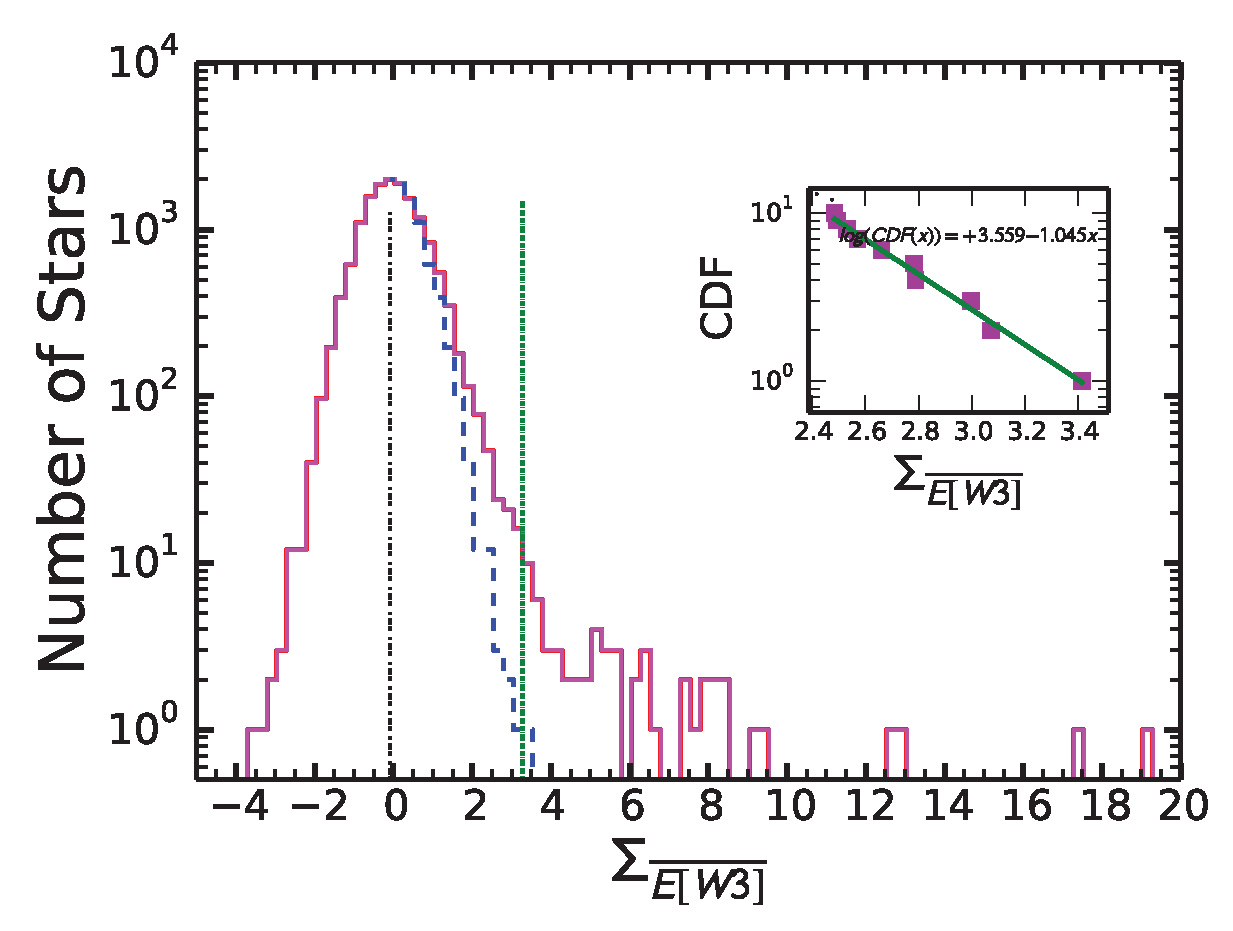
\includegraphics[scale=0.4]{Ch4/W3Joint_colordist_bgt5}&
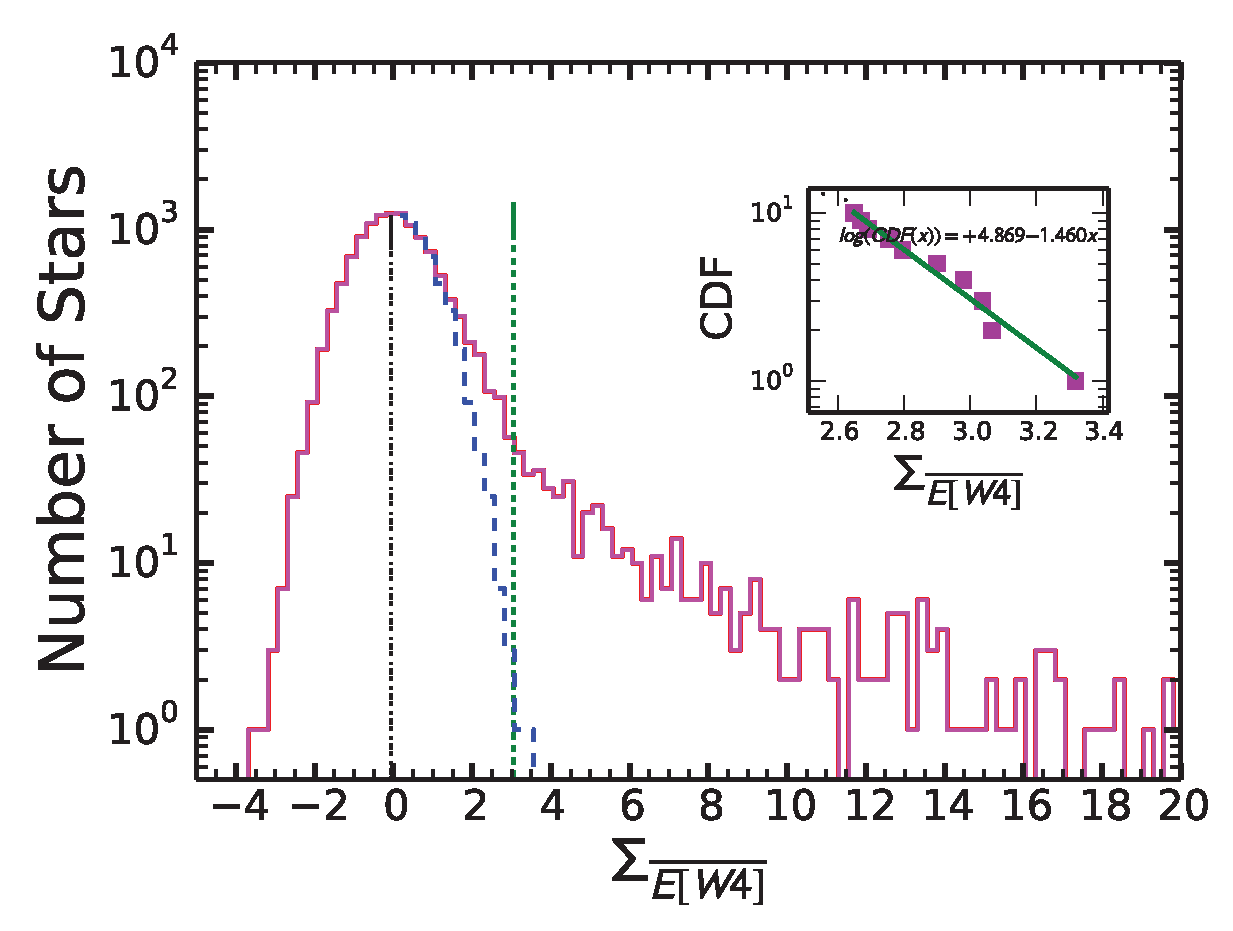
\includegraphics[scale=0.4]{Ch4/W4_All3_Joint_colordist_bgt5}
\end{tabular}
\caption[Weighted Excess $\Sigma_{\overline{E}}$ Distributions]{Distributions of the weighted-excess metrics, $\Sigma_{\overline{E[W3]}}$ (left) and $\Sigma_{\overline{E[W4]}}$ (right) for all stars in our parent sample. We have assumed that the negative portion of each \ES\ distribution is representative of the intrinsic random and systematic noise in the data (Section~\ref{sec:improved_detection}). The mode of the full distribution is shown by a vertical black dashed-dot line. A reflection (dashed histogram) of the negative portion of the \ES\ histogram around the mode is thus representative of the false positive excess expectation. We define the FDR at a given \ES\ as the ratio of the cumulative numbers of $>$\ES\ excesses in the positive tails of the dashed and solid histograms.  The vertical dotted lines indicate the FDR thresholds for each weighted-$Wj$ excess, 2\% for $W3$ and 0.5\% for $W4$, above which we identify all stars as probable debris disk hosts. Each inset shows a log-log fit of a line to the last ten points in the reverse cumulative distribution function of the uncertainties (see Section~\ref{sec:improved_detection}). This fit smoothes over the stochasticity in this sparsely populated region of the uncertainty distribution to attain a more accurate estimate of the FDR threshold.}
\label{fig:ColorDist}
\end{figure}



\begin{figure}
\centering
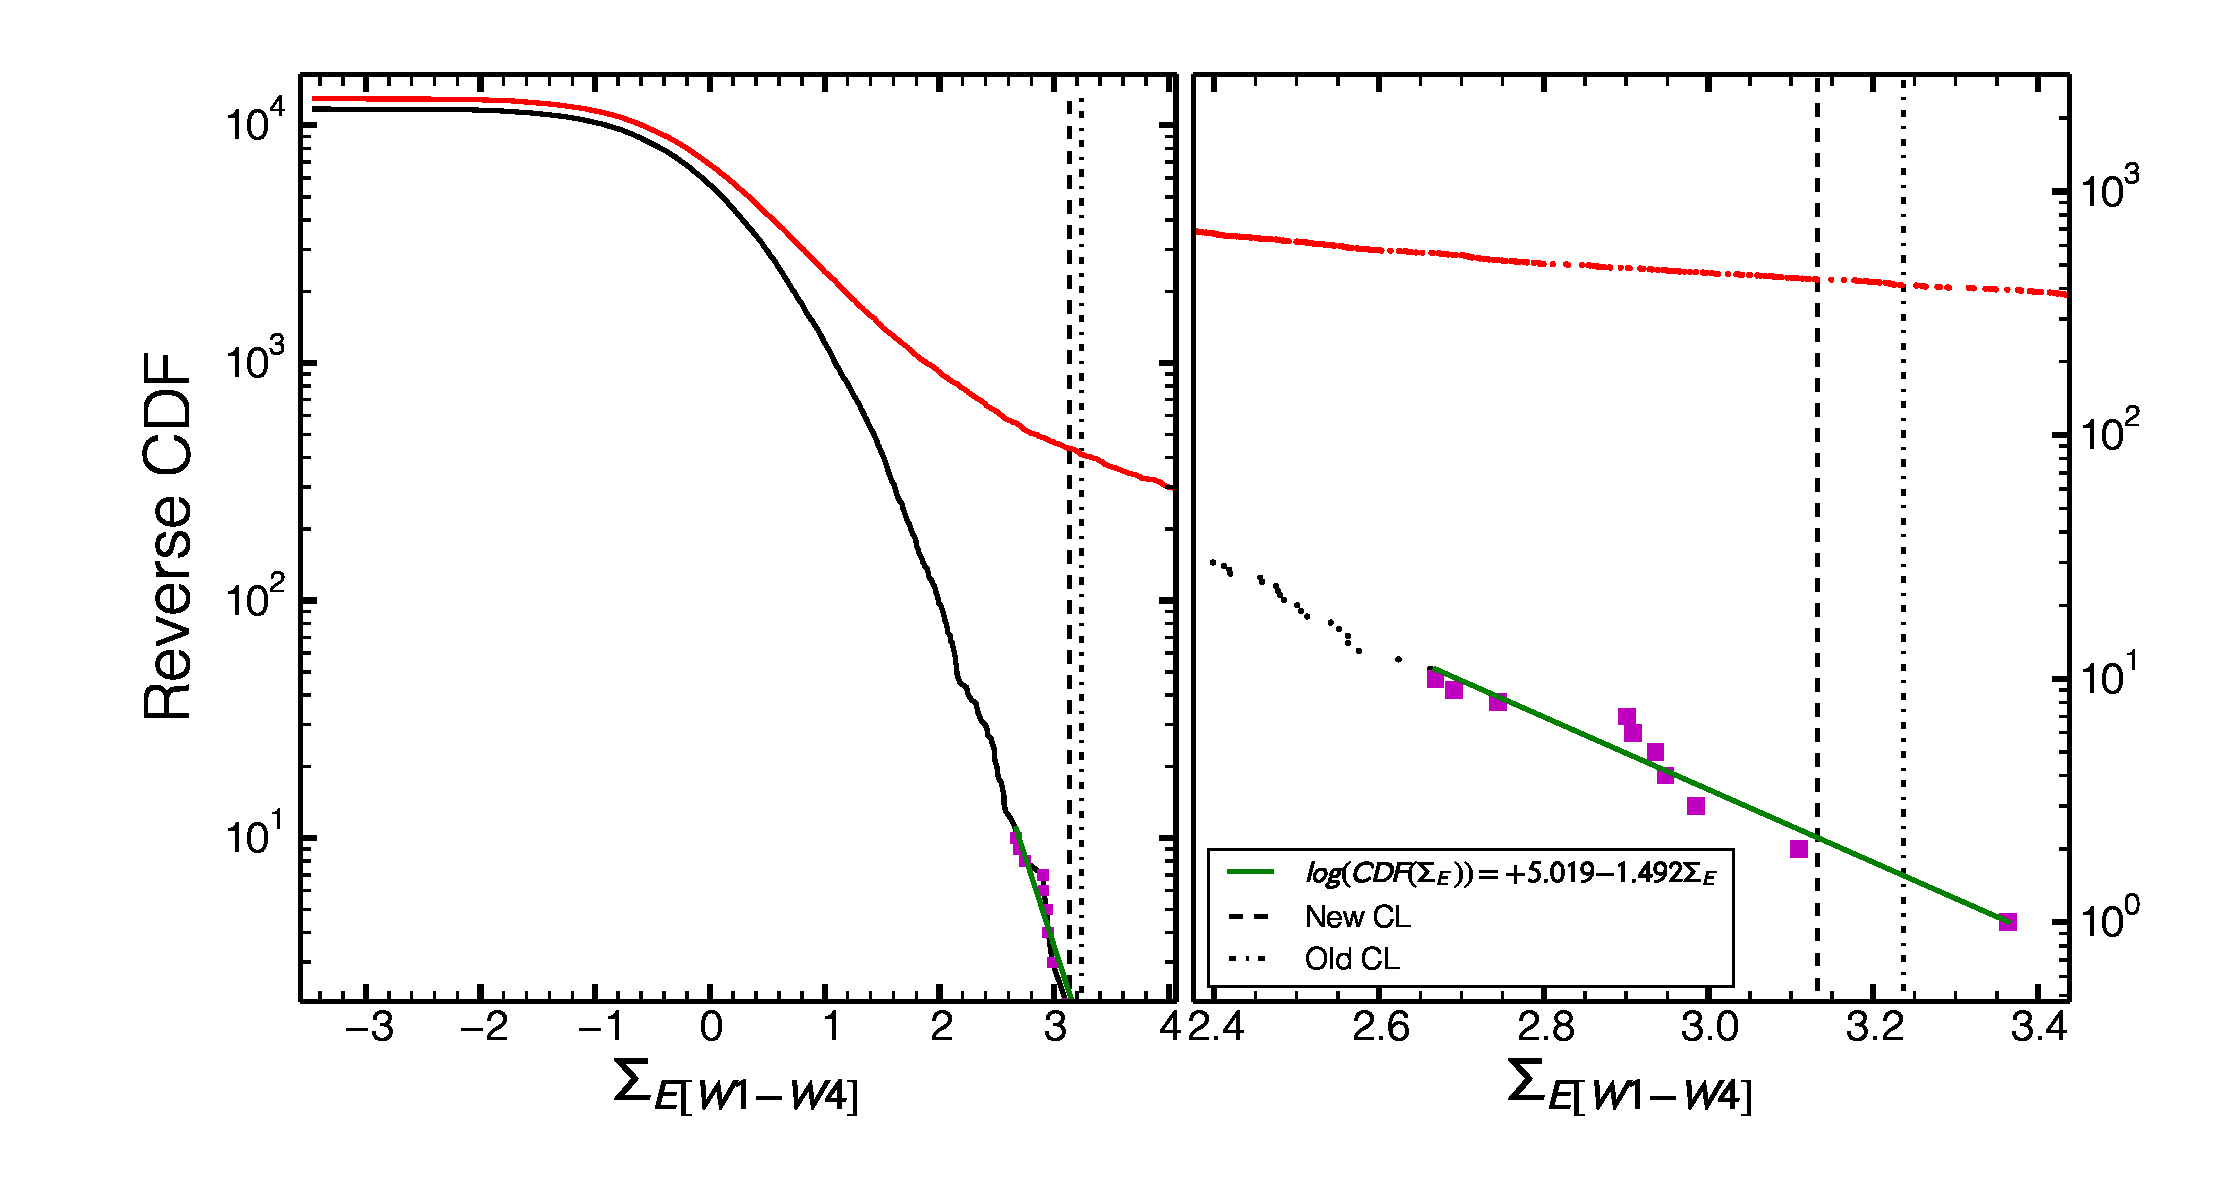
\includegraphics[scale=0.4]{Ch4/CL_Comparison}
\caption[Improved Assessment of False Discovery Rate]{A reverse cumulative distribution function (rCDF, Section~\ref{sec:improved_detection}) of the uncertainty (black) and excess (red) distributions of $\Sigma_{E[W1-W4]}$. We use the rCDF to estimate the FDR at any $\Sigma_E$: as the ratio of the black and red rCDFs. The vertical dash-dotted line shows the more conservative $\Sigma_{E_{99.5}}$ estimate of the confidence threshold, from \p14.  The vertical dashed line shows the present, more accurate, $\Sigma_{E_{99.5}}$ estimate, based on a fit (solid green line) to the last ten data points in the tail of the rCDF (magenta squares). The left panel shows the full rCDFs, while the right panel zooms in near the $\Sigma_{E_{CL}}$ threshold.} 
\label{fig:CL_Comparison}
\end{figure}



\begin{figure}
\centering
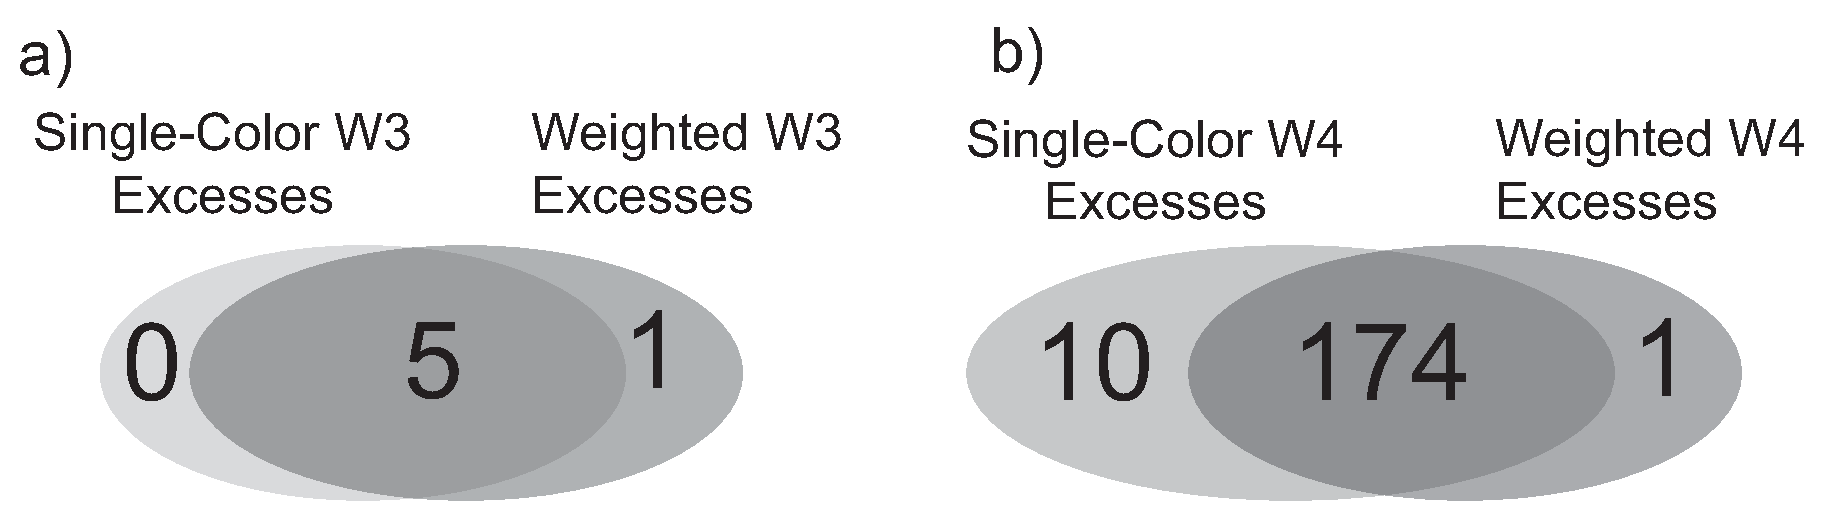
\includegraphics[scale=0.5]{Ch4/Venn_wtdvsSingle}
\caption[Venn Diagram of \WS\ weighted- and single-color Excesses.]{Venn diagrams comparing the candidate excesses from our weighted-excess analysis (right circles) and from our single-color excess (left circles). Stars from the single-color excess sets were selected only if they had good quality photometry in $W1$, $W2$ and $W3$ for our $W3$ excesses (a) and good quality photometry in all four bands for our $W4$ excesses (b).}
\label{fig:Venn}
\end{figure}


\begin{figure}
\centering
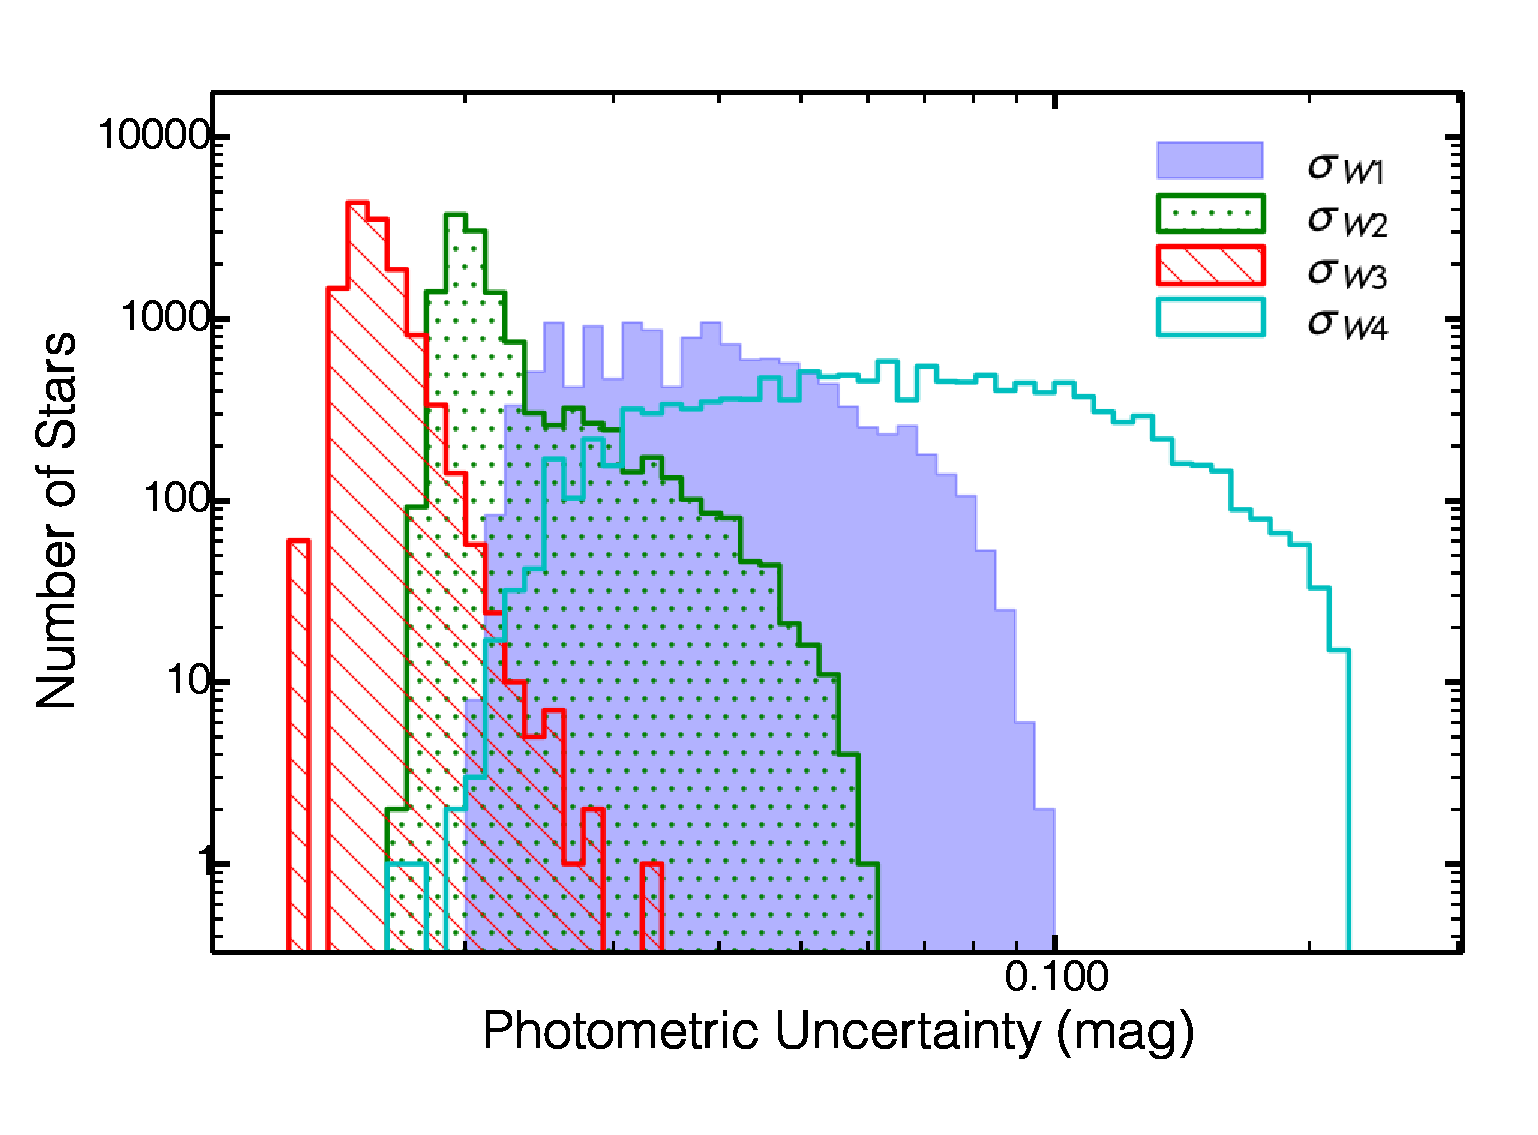
\includegraphics[width=\textwidth]{Ch4/uncdist_psample}
\caption{Distributions of photometric uncertainties for all four \WS\ bands for 12654 stars in the weighted $W4$ parent sample, including stars with saturated and then corrected $W1$ and $W2$ photometry. The large spread in $\sigma_{W4}$ is expected because of the lower absolute flux levels in $W4$. It is evident that the mean $\sigma_{W1}$ is larger than that for $\sigma_{W2}$ and $\sigma_{W3}$. This systematic trend of increasing photometric uncertainty from $W3$ down to $W1$ dominates the determination of a significant excess when the $E[Wi-Wj]$ are comparable.}
\label{fig:wise_errors}
\end{figure}


\begin{figure}
\centering
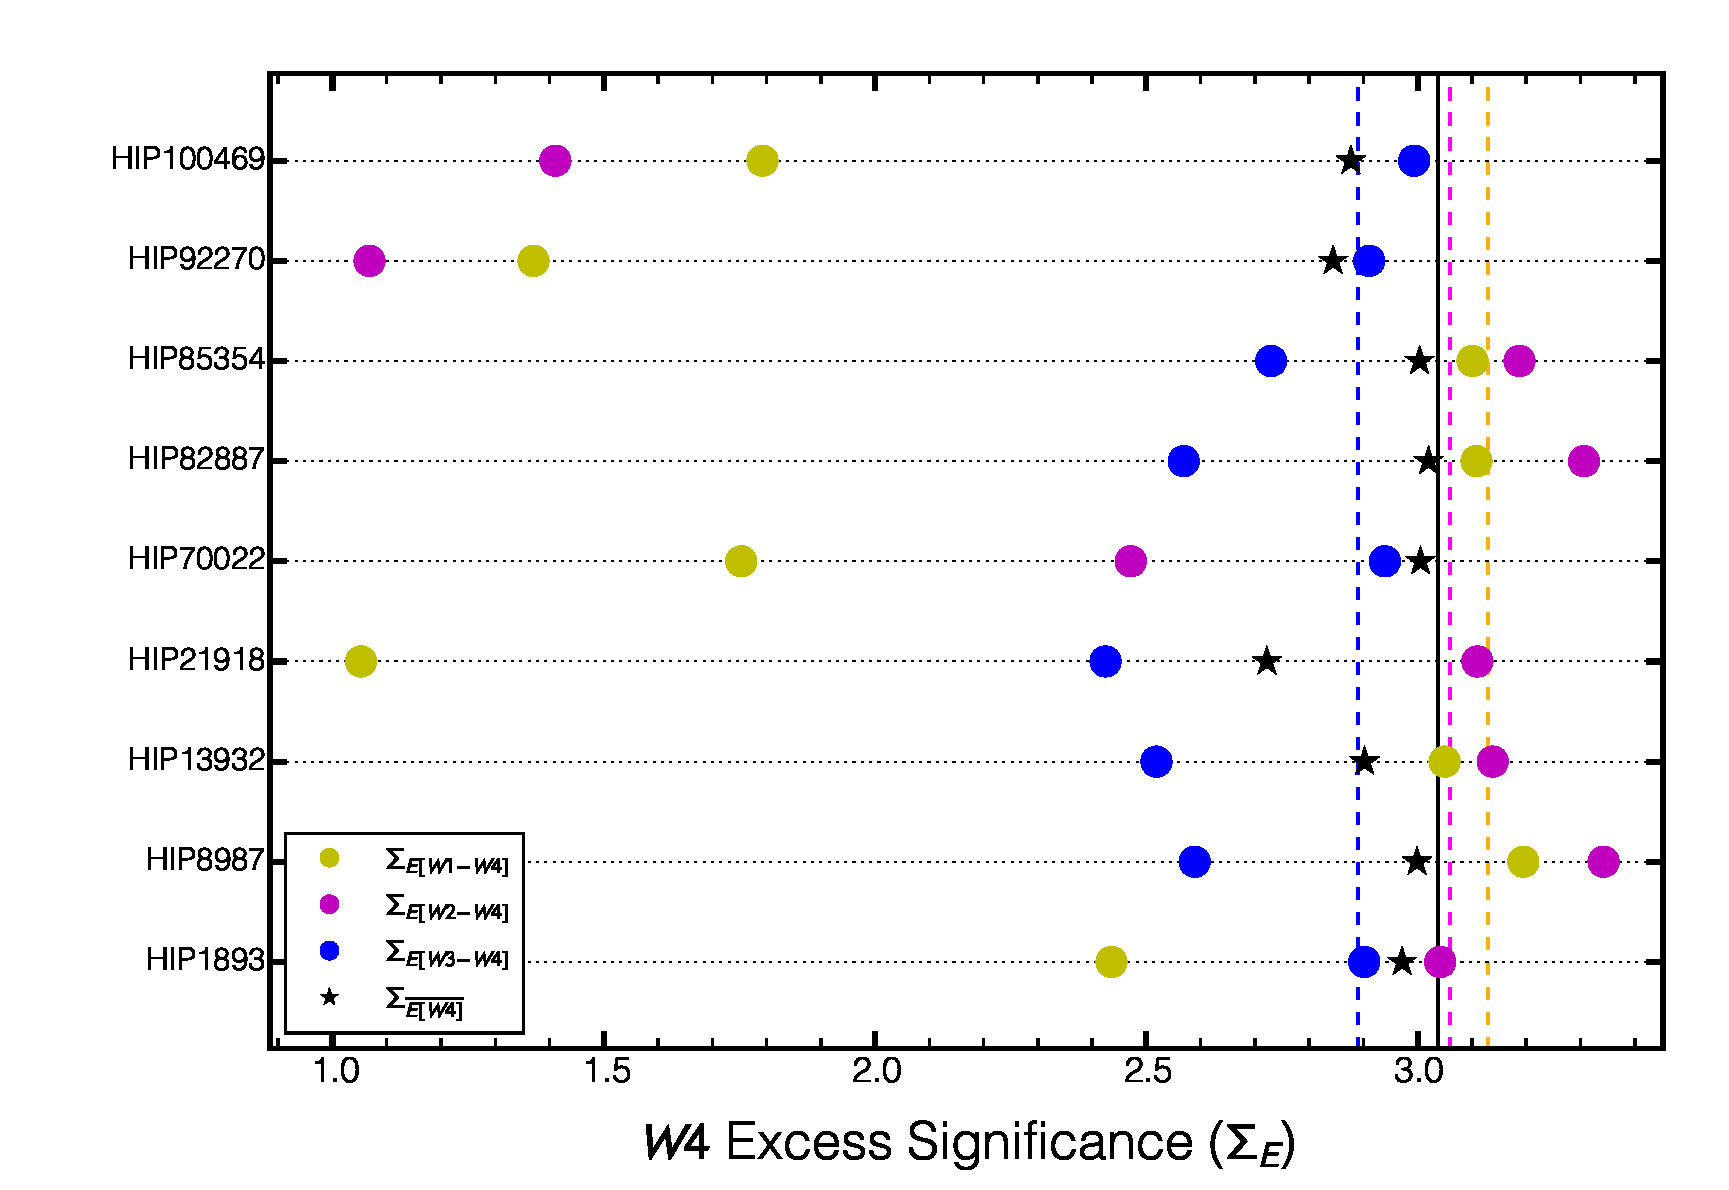
\includegraphics[scale=0.5]{Ch4/Unrecovered_10}
\caption{The excess significances for the nine stars with single-color $W4$ excesses in \p14 that were not recovered with the weighted-$W4$ excess metric in this study (see Figure~\ref{fig:Venn}b). Each vertical colored line corresponds to the current 99.5\% detection threshold for each color listed in the legend. We see that the weighted-$W4$ excess threshold ($\Sigma_{\overline{E[W4]}}$ effectively averages the individual single-color detection thresholds.}
\label{fig:unrecovered_10}
\end{figure}

\begin{figure}
\centering
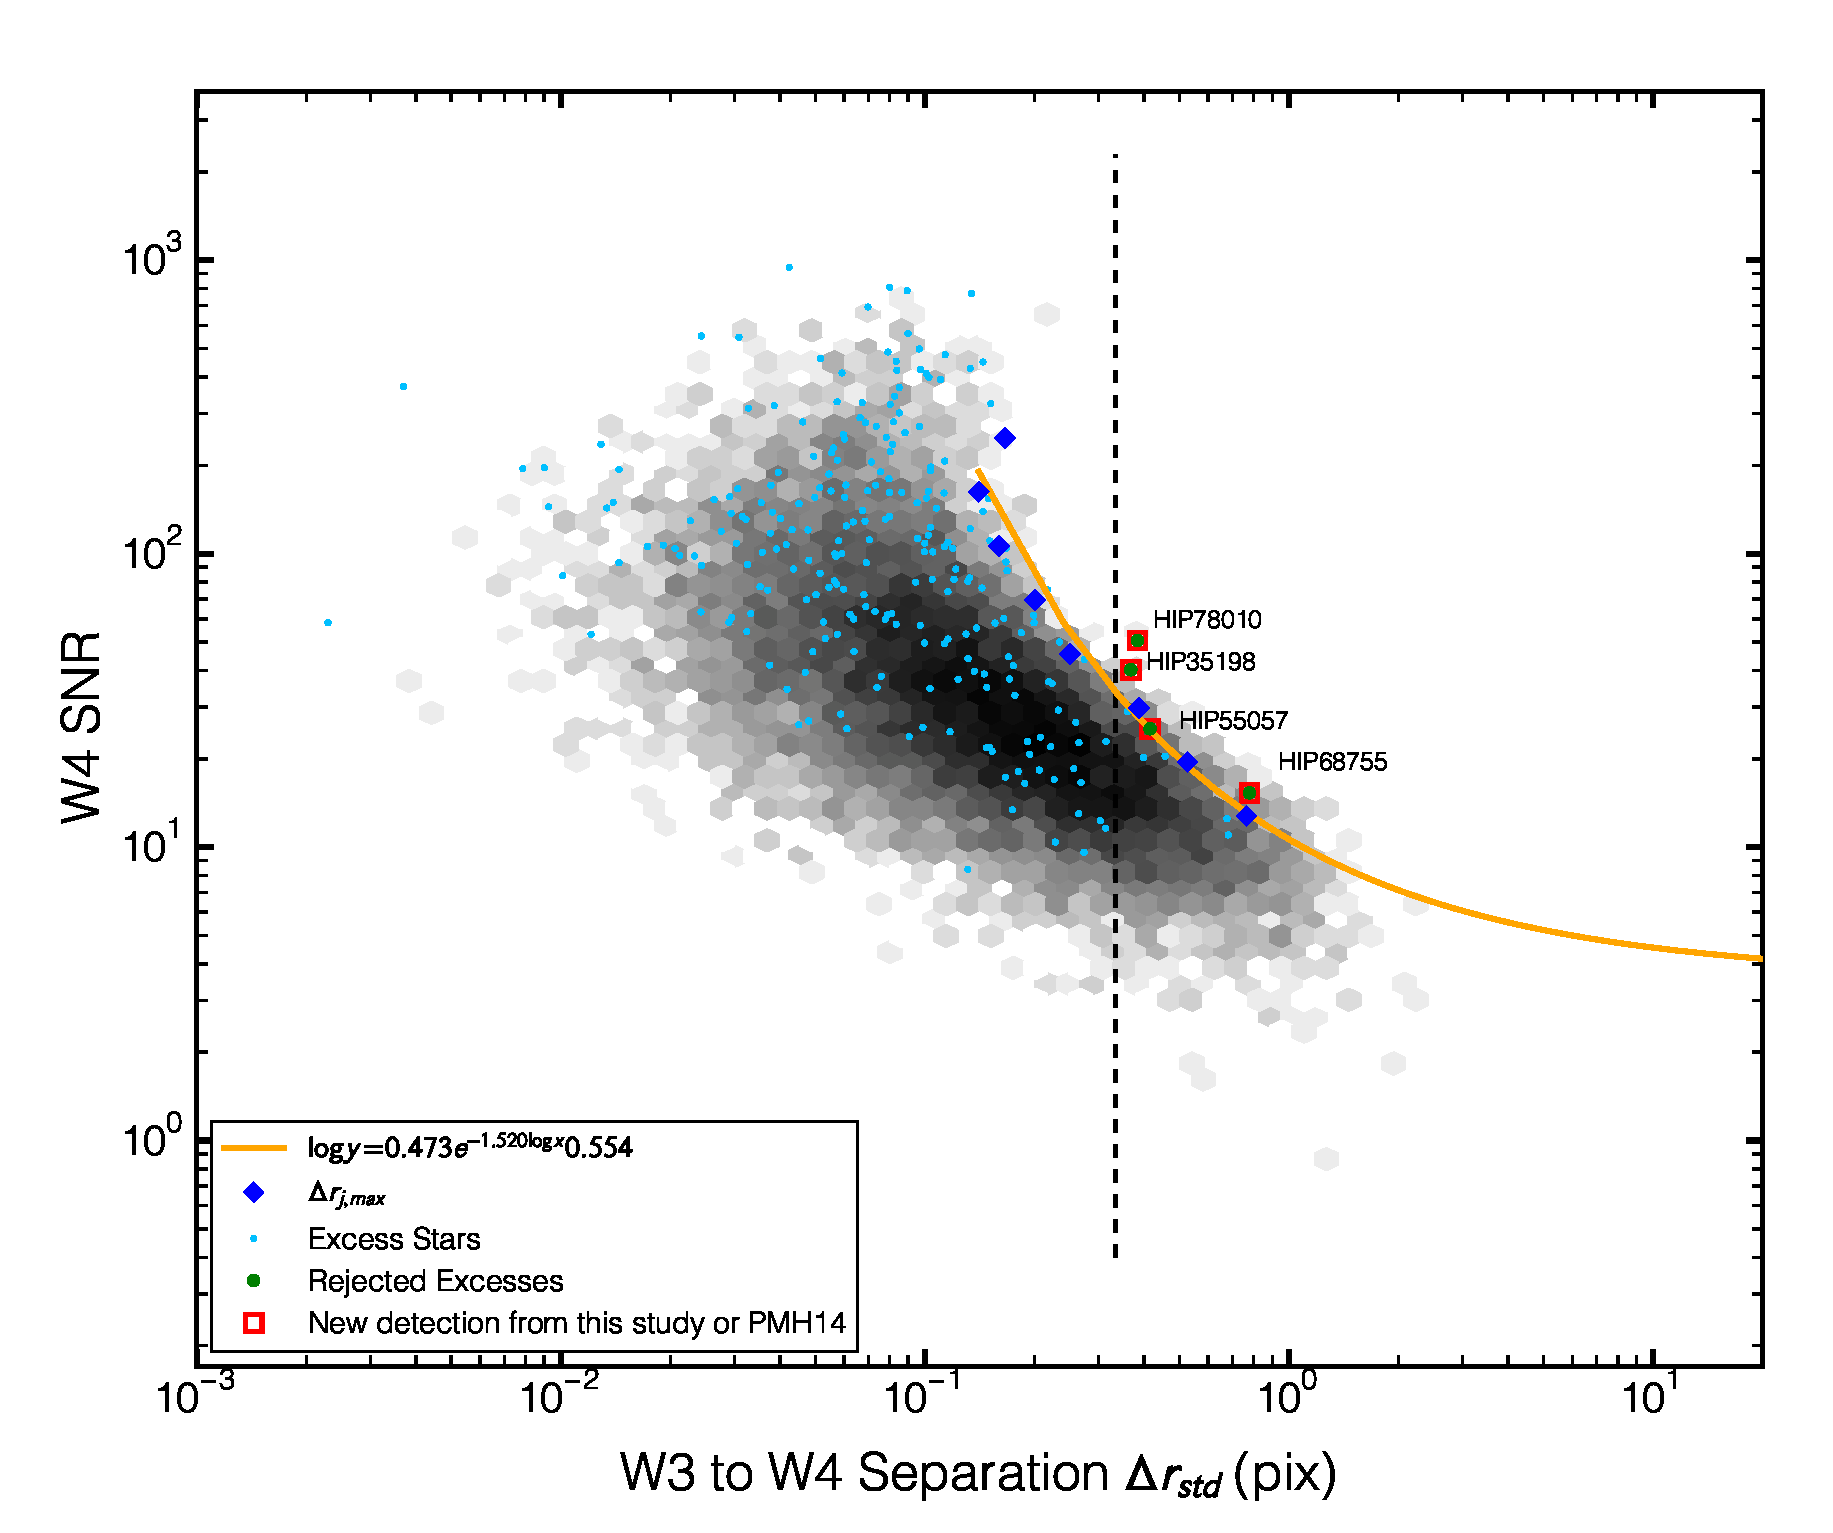
\includegraphics[scale=0.5]{Ch4/w3w4_snrvsep}
\caption{Distribution of relative positional offsets of stellar centroids between $W3$ and $W4$ using images from the \textit{unWISE} image service, plotted with respect to the $W4$ SNR calculated from the \textit{unWISE} images. The black/gray density cloud represents the density of 16927 Hipparcos stars from the parent 120~pc sample, while the light-blue dots show the locations of our excess stars. The black-dotted line represents our separation cut-off ($1/3$~pixels) below which stars are not rejected. Our rejection threshold (orange dotted line) was fit to $\{\Delta r_{j,max}\}$ (dark-blue diamonds), calculated as described in Section~ \ref{sec:unwise_rejectmethod}. Excesses to the right of the vertical dotted black line and above the orange dotted line (red squares) are identified by name and deemed to be contaminated by an unrelated nearby point or extended source seen in projection.}


\label{fig:w3w4_snrvsep}
\end{figure}

\begin{figure}
\centering
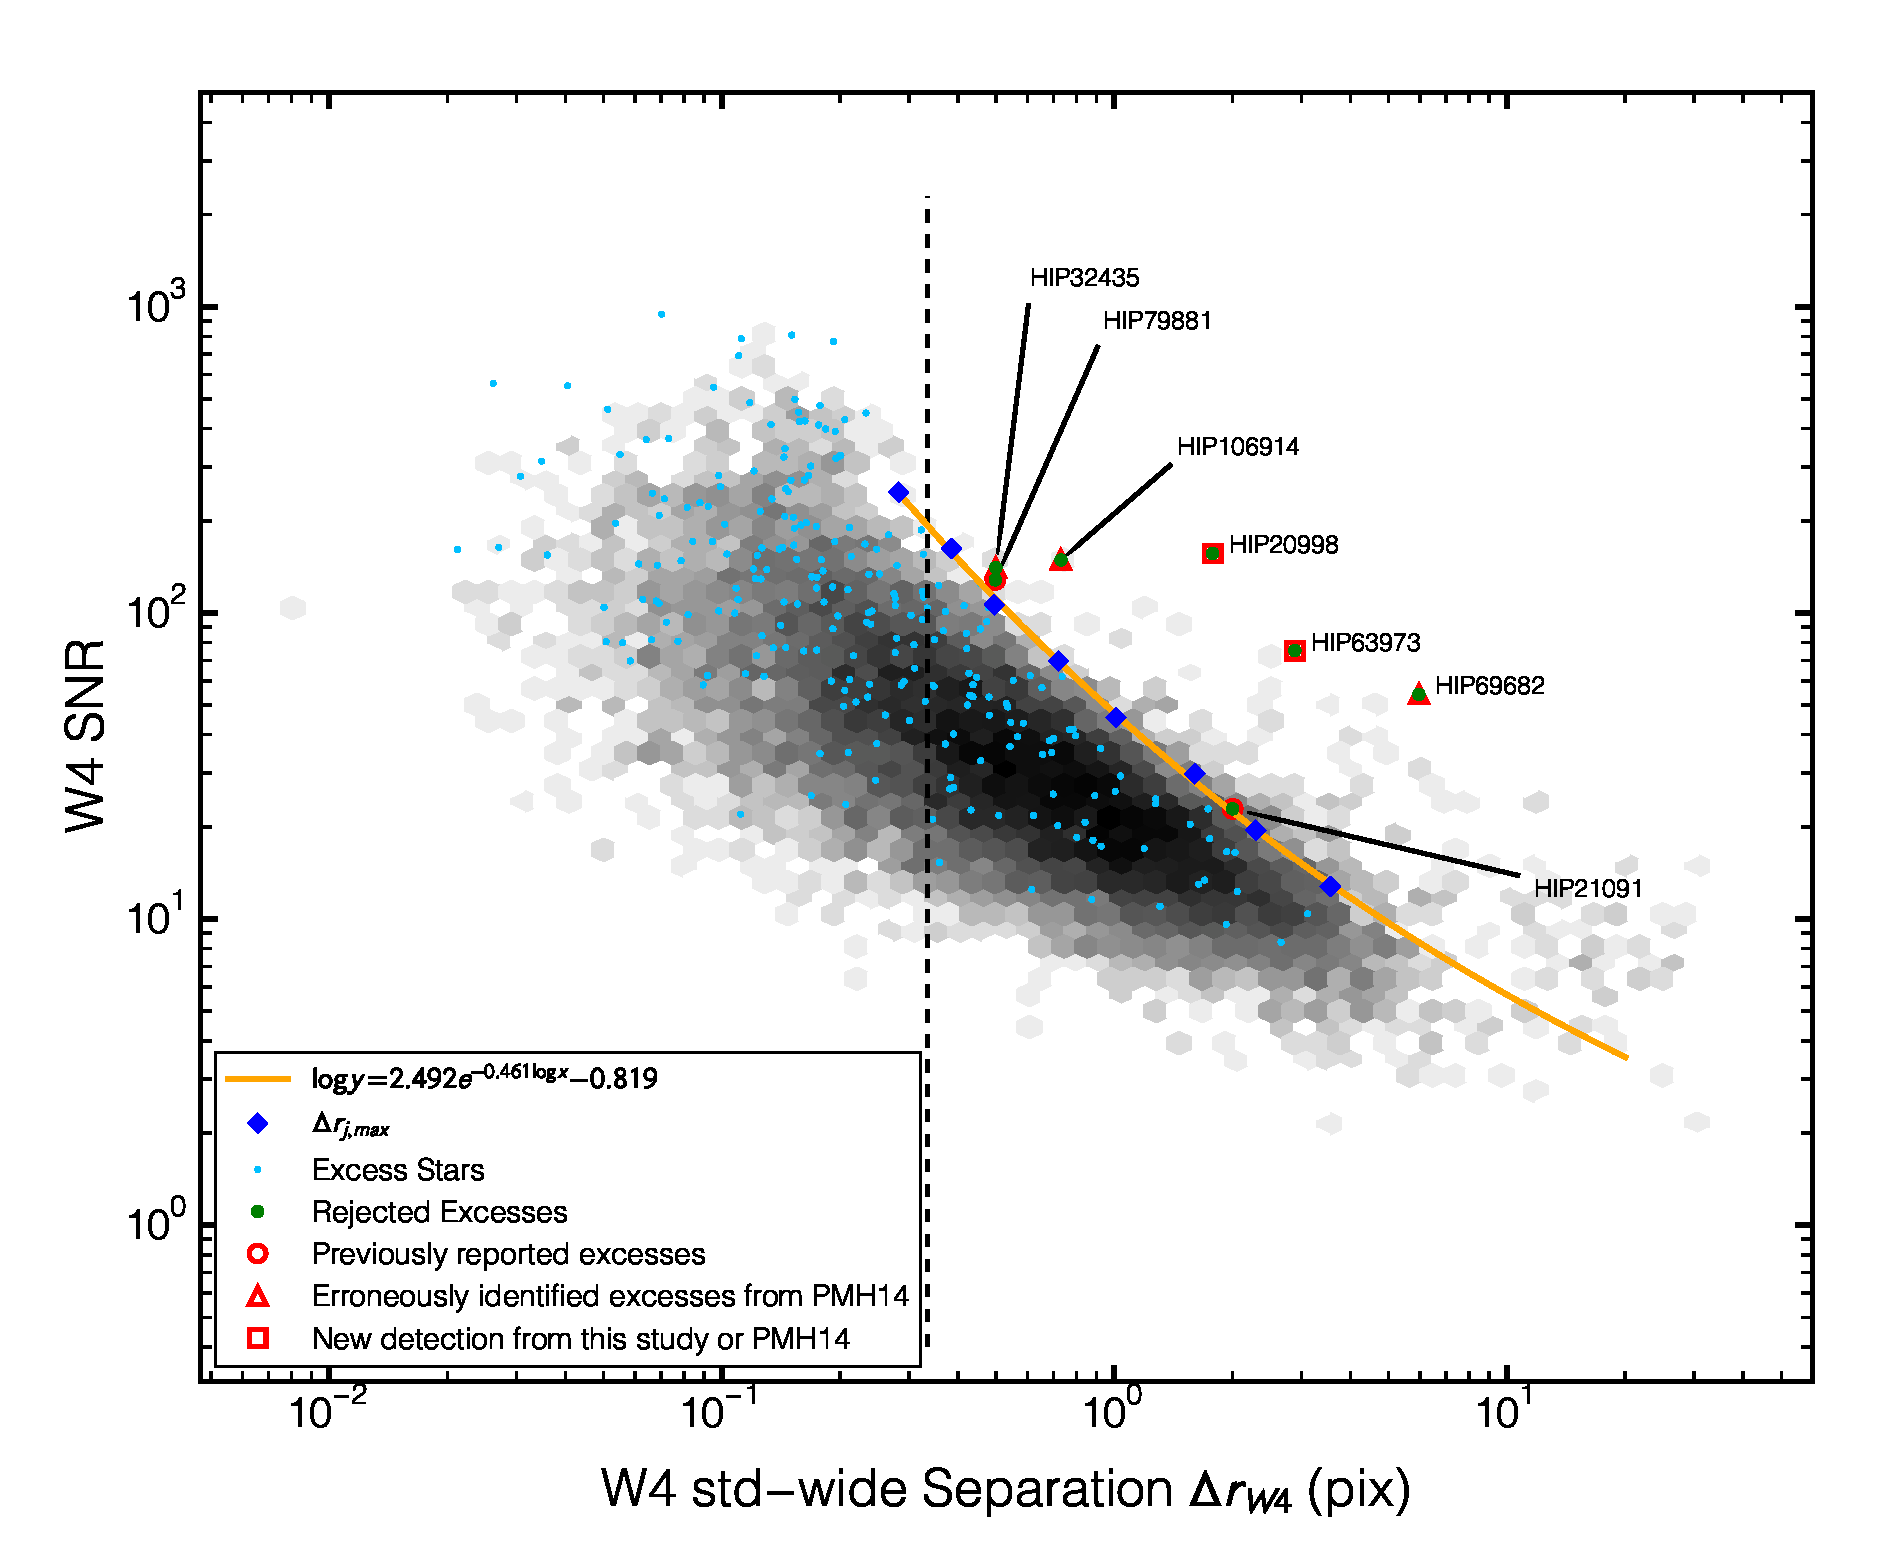
\includegraphics[scale=0.5]{Ch4/w4w4_snrvsep}
\caption{Distribution of relative positional offsets of stellar centroids between a narrow 2.5~pixel radius and wide 10~pixel radius apertures, as described in Section~\ref{sec:centroid_calc}. The plot elements are the same as those described in Figure~\ref{fig:w3w4_snrvsep}. Excesses to the right of the vertical dotted black line and above the orange dotted line (red squares, circles, and triangles) are identified by name and deemed to be contaminated by an unrelated nearby point or extended source seen in projection.}
\label{fig:w4w4_snrvsep}
\end{figure}

\begin{figure}
\centering
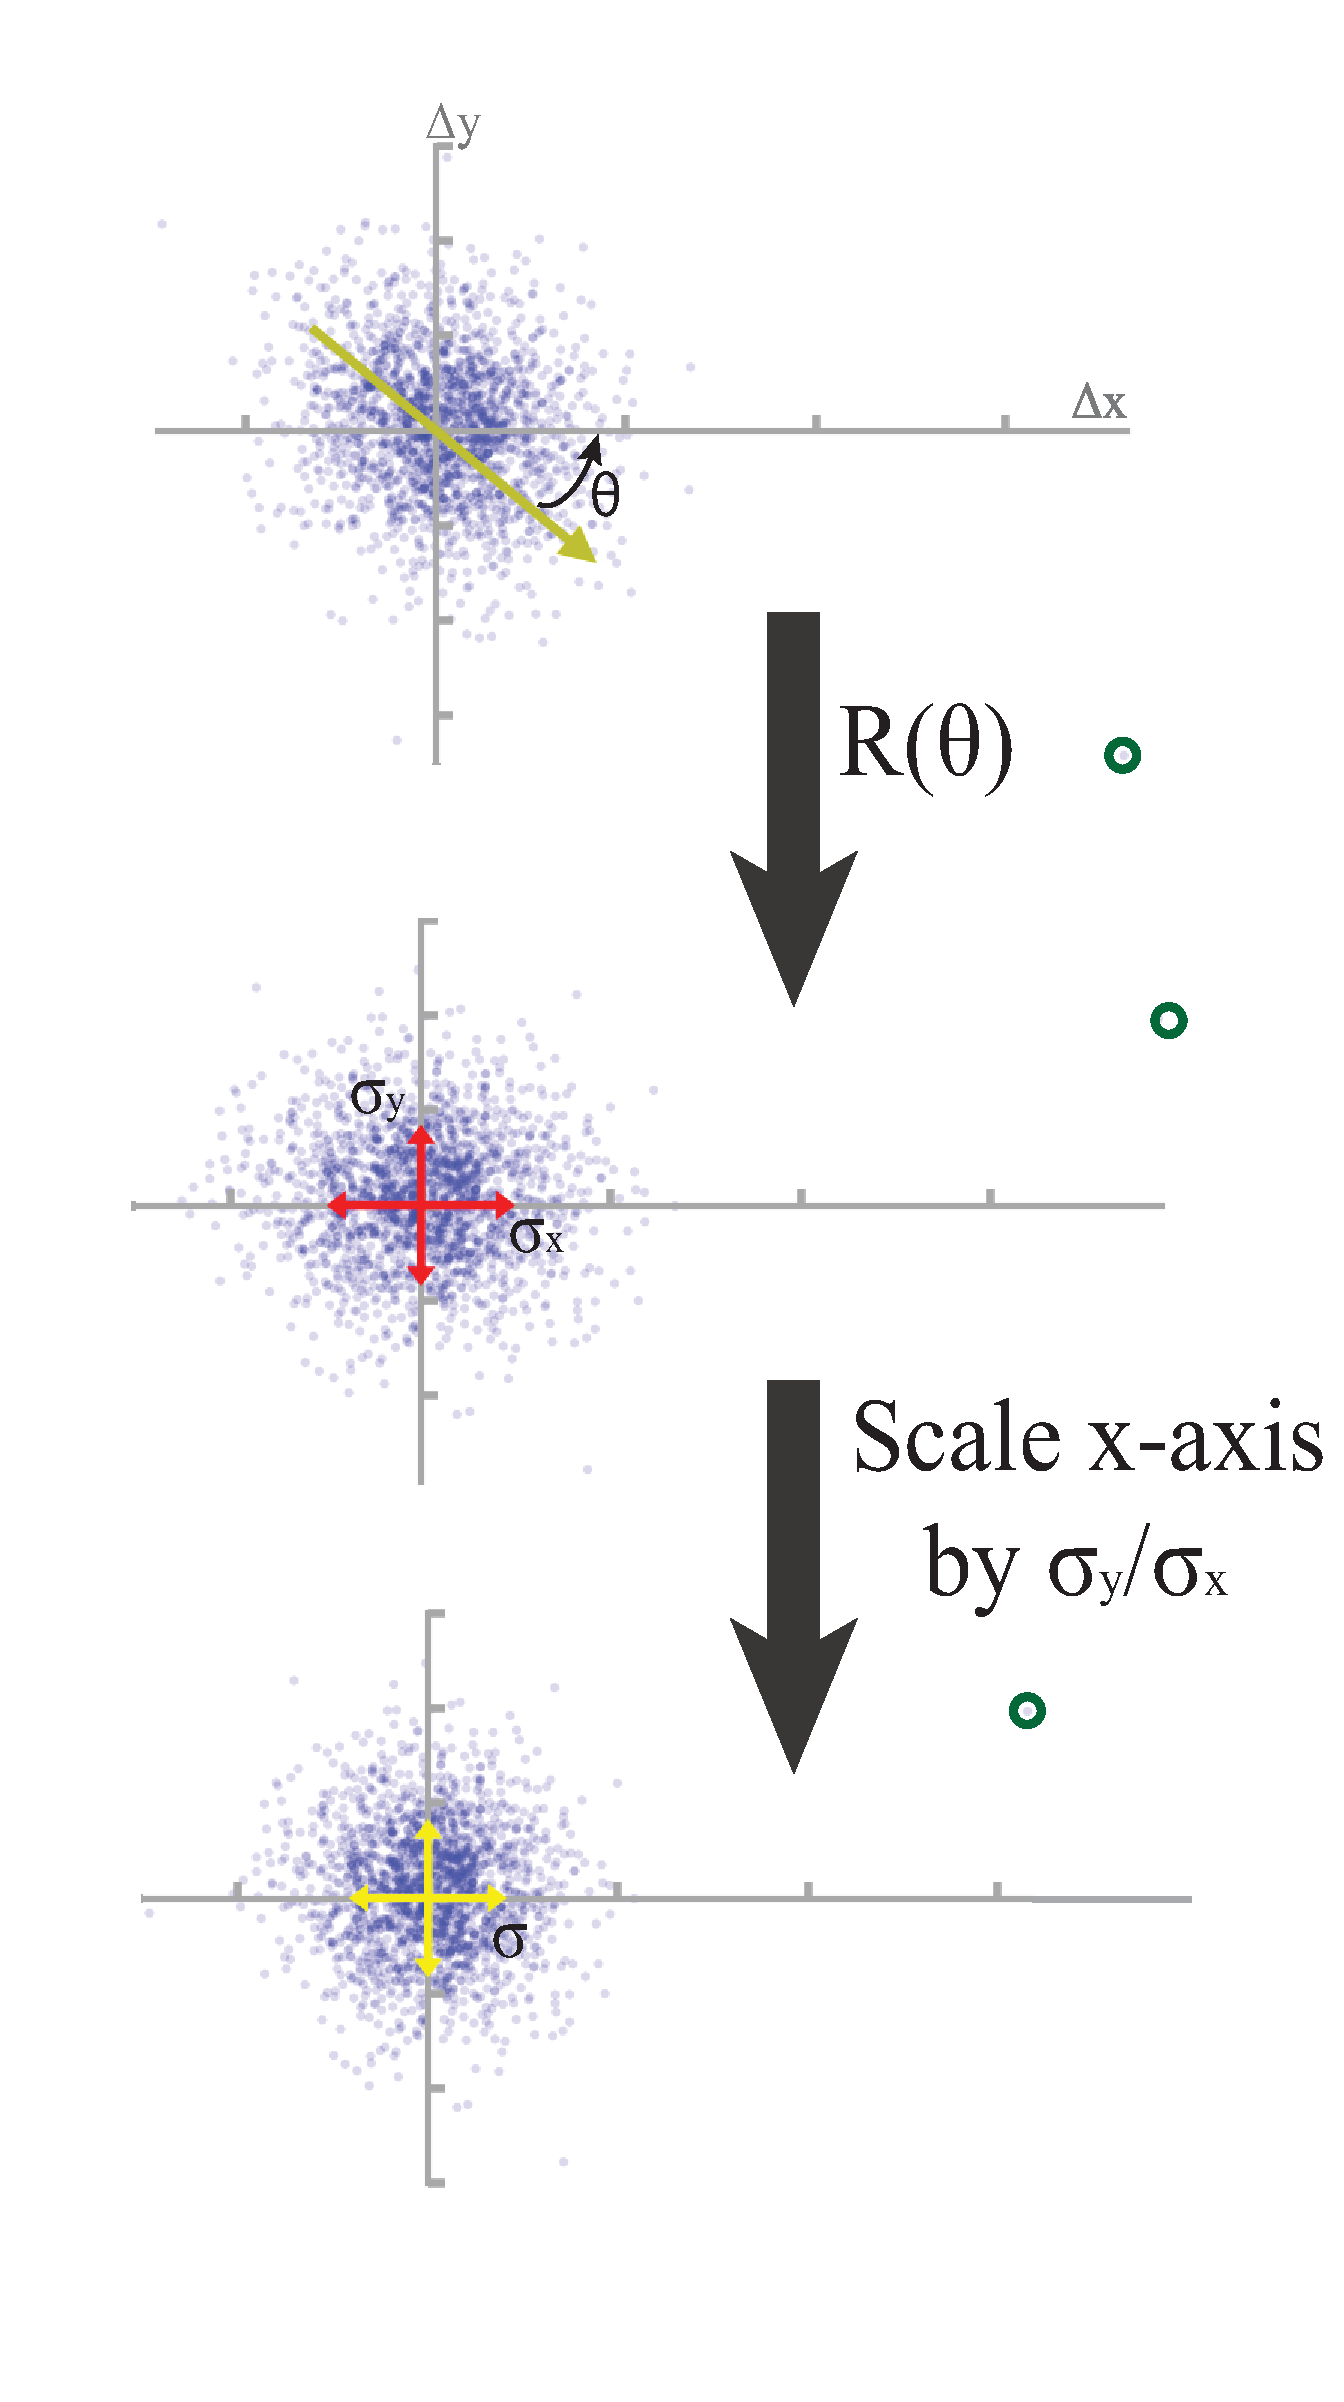
\includegraphics[scale=0.45]{Ch4/unwise_transform_python} 
\caption{An illustration to show the procedure of circularizing the 2-Dimensional $\Delta x$ vs. $\Delta y$ centroid offset distributions for each $j^{th}$ SNR bin. The illustration shows the transformation of data in the $W4$ SNR bin $= [55:84]$ in the $\Delta r_{W3,W4}$ vs. $W4$ SNR analysis. A detailed description of each step can be found in Section~\ref{sec:unwise_rejectmethod}. The purpose of this procedure is to obtain a simple theoretical form of the behavior of the core of the 2-Dimensional distribution to determine the position of $\Delta r_{j,max}$. We de-rotated the distribution by $\theta$, which we obtained from the first principal component vector of the distribution and then scaled the rotated $x$-axis by the ratio of the minor to major axes lengths (i.e., standard deviations along $\Delta x$ and $\Delta y$). We then fit a 2-D Gaussian surface to obtain $\sigma_j$ which allows us to transform an elliptical Gaussian to an azimuthally symmetric Gaussian. The reader can observe the open green circle to follow the transformation from panel to panel.}
\label{fig:unwise_transform}
\end{figure}


\begin{figure}
\centering
\begin{tabular}{c}
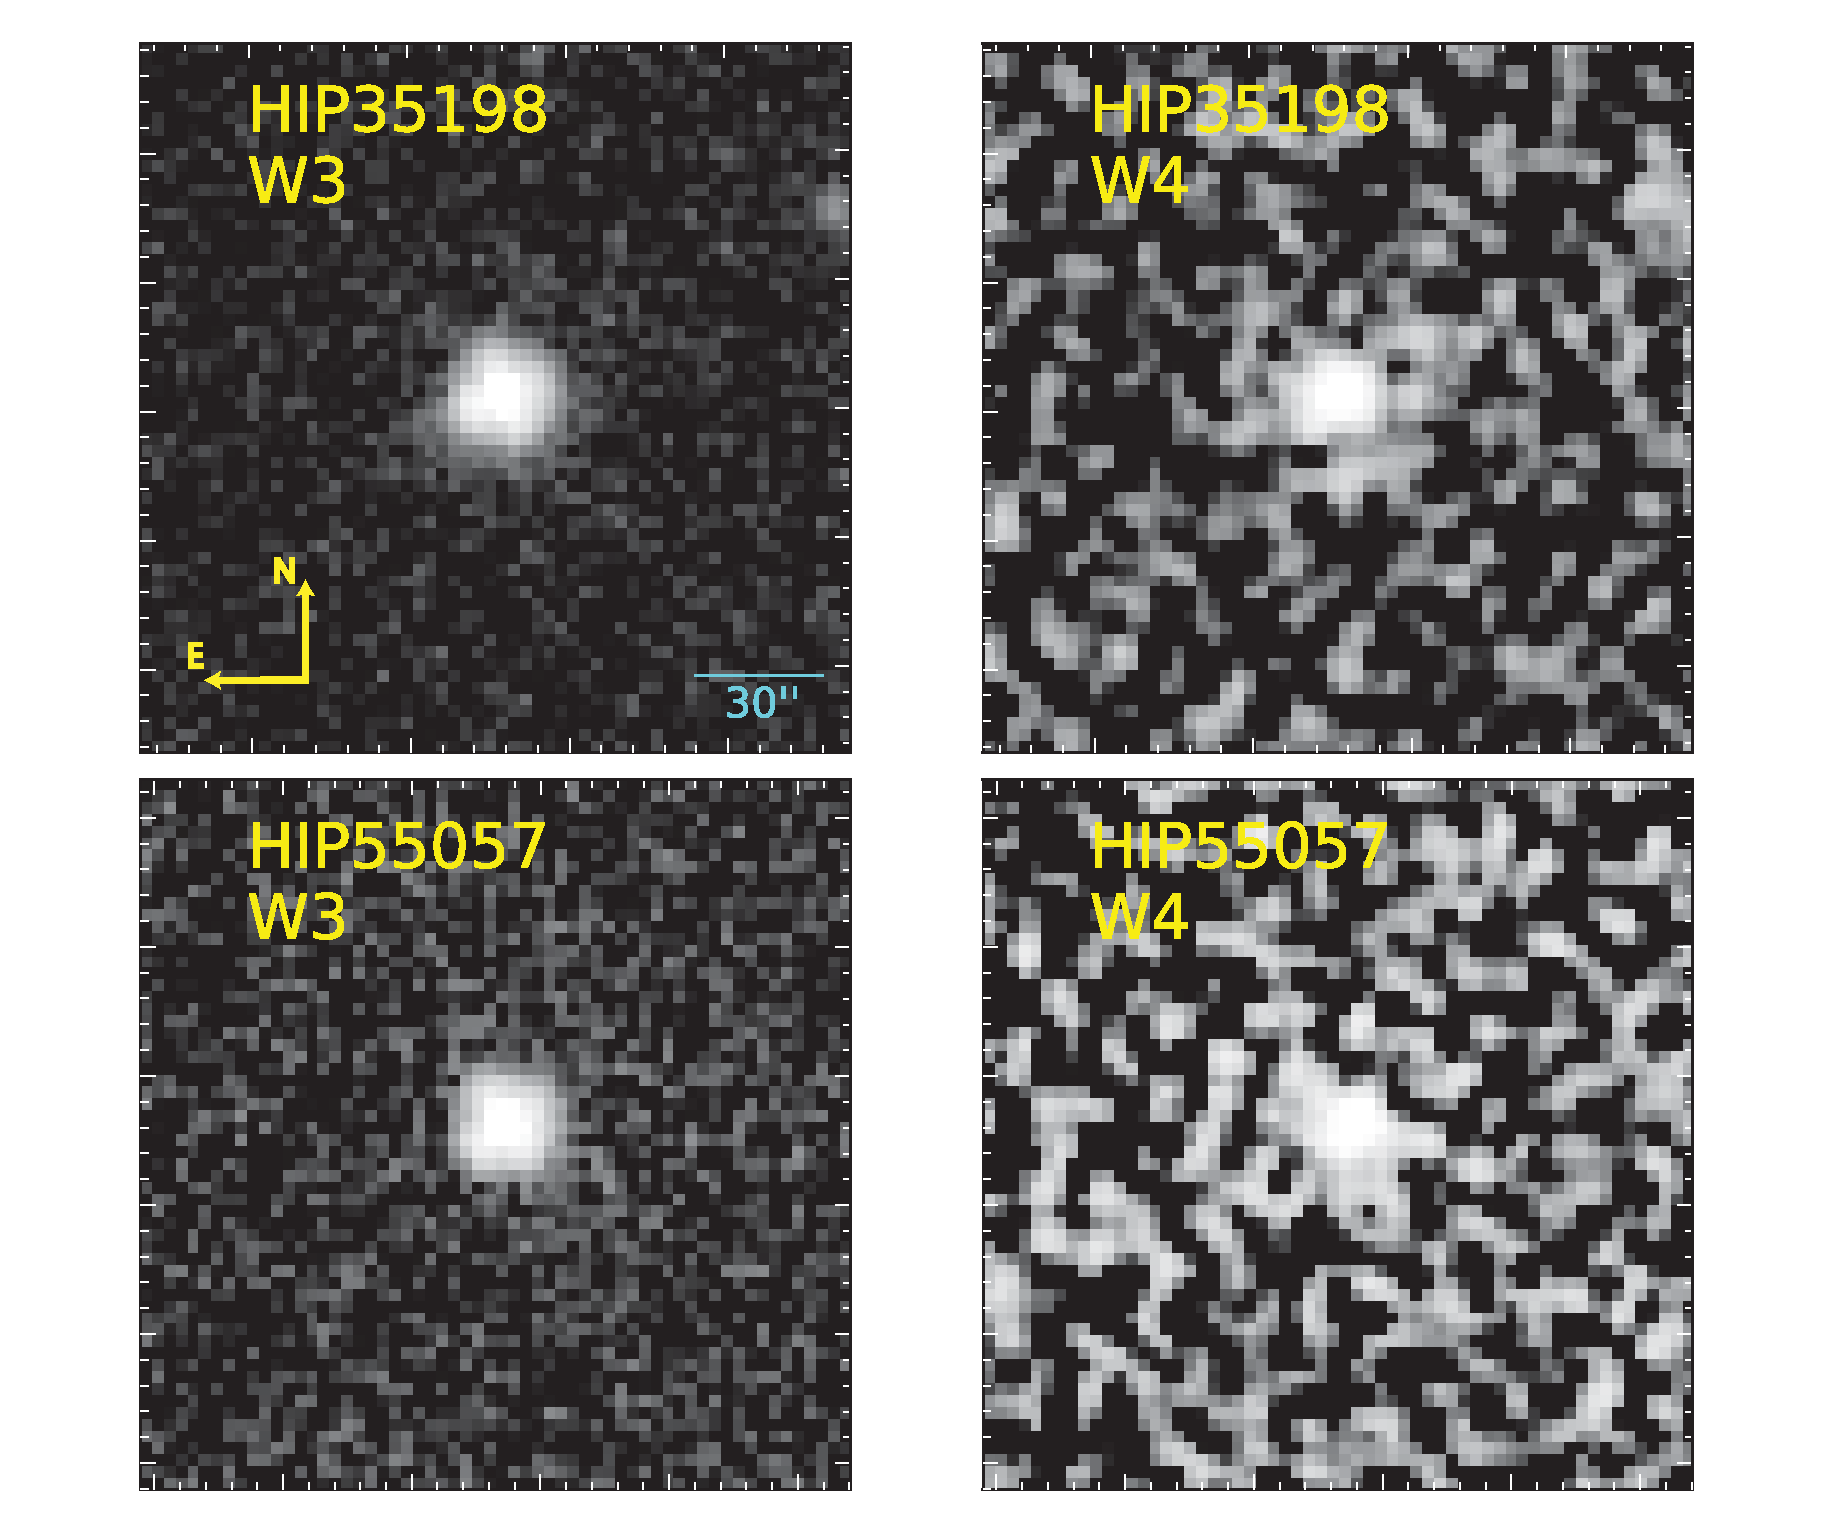
\includegraphics[width=0.7\textwidth]{Ch4/W3W4_rejected_postagestamps_1}\\
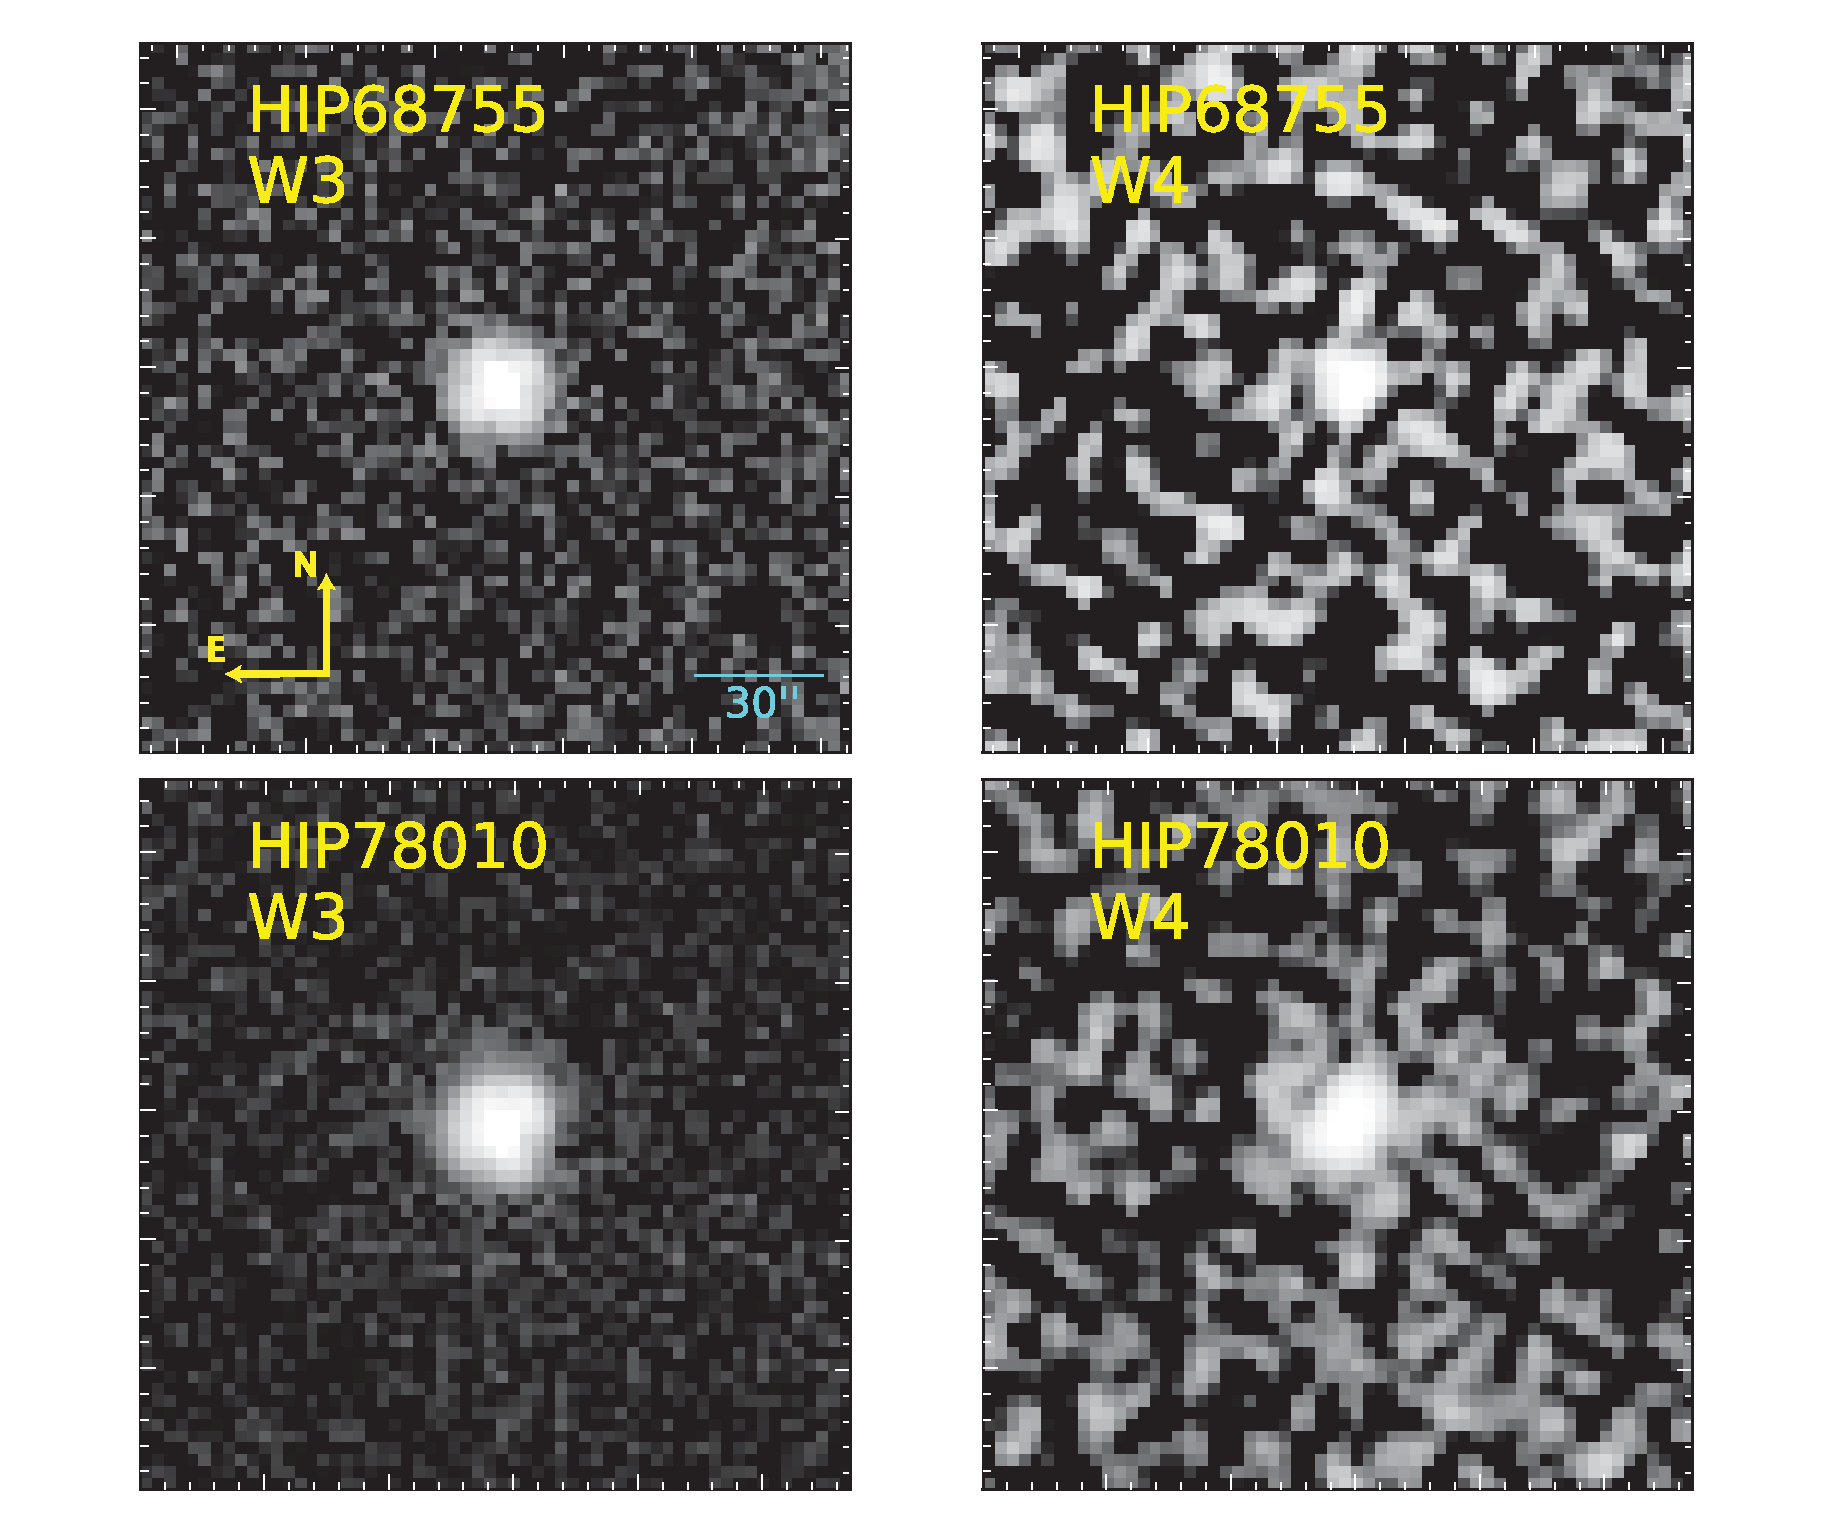
\includegraphics[width=0.7\textwidth]{Ch4/W3W4_rejected_postagestamps_2}
\end{tabular}
\caption{1'$\times$1' \textit{unWISE} $W3$ and $W4$ postage stamp images of stars rejected by our point-source contamination ($\Delta r_{W4}$ vs. $W4$ SNR) analysis. The images are displayed using an ArcSinh scale.}
\label{fig:w3w4_postagestamps}
\end{figure}


\begin{figure}
\centering
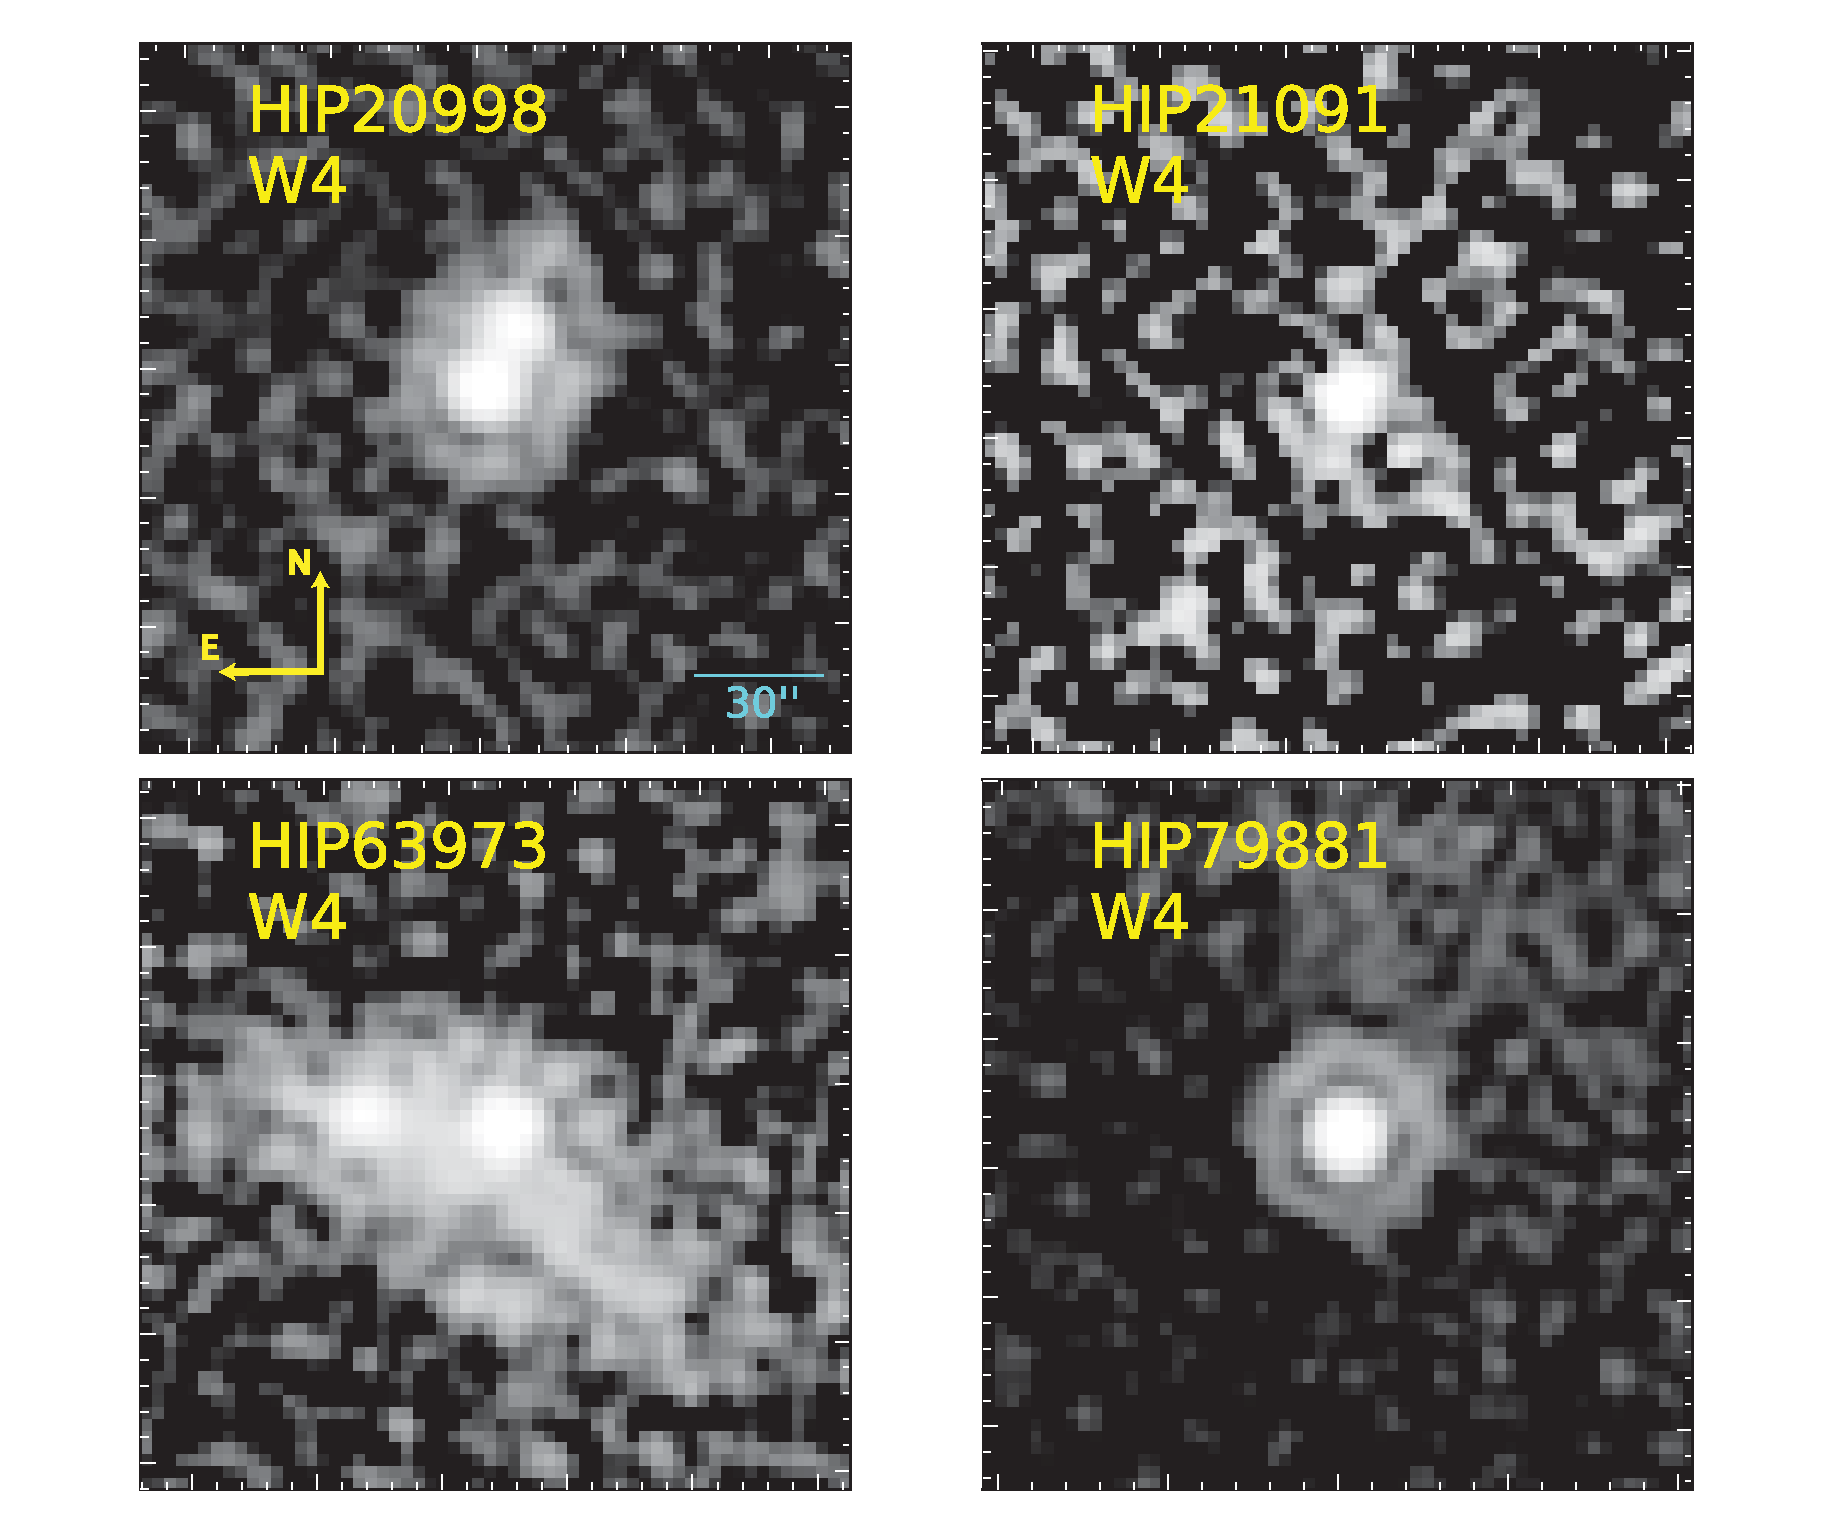
\includegraphics[scale=0.5]{Ch4/W4W4_rejected_postagestamps}
\caption{1'$\times$1' \textit{unWISE} $W4$ postage stamp images of stars rejected from our extended emission contamination ($\Delta r_{W4}$ vs. $W4$ SNR) analysis. The images are displayed using an ArcSinh scale.}
\label{fig:w4w4_postagestamps}
\end{figure}





\begin{figure}
\centering
\begin{tabular}{cc}
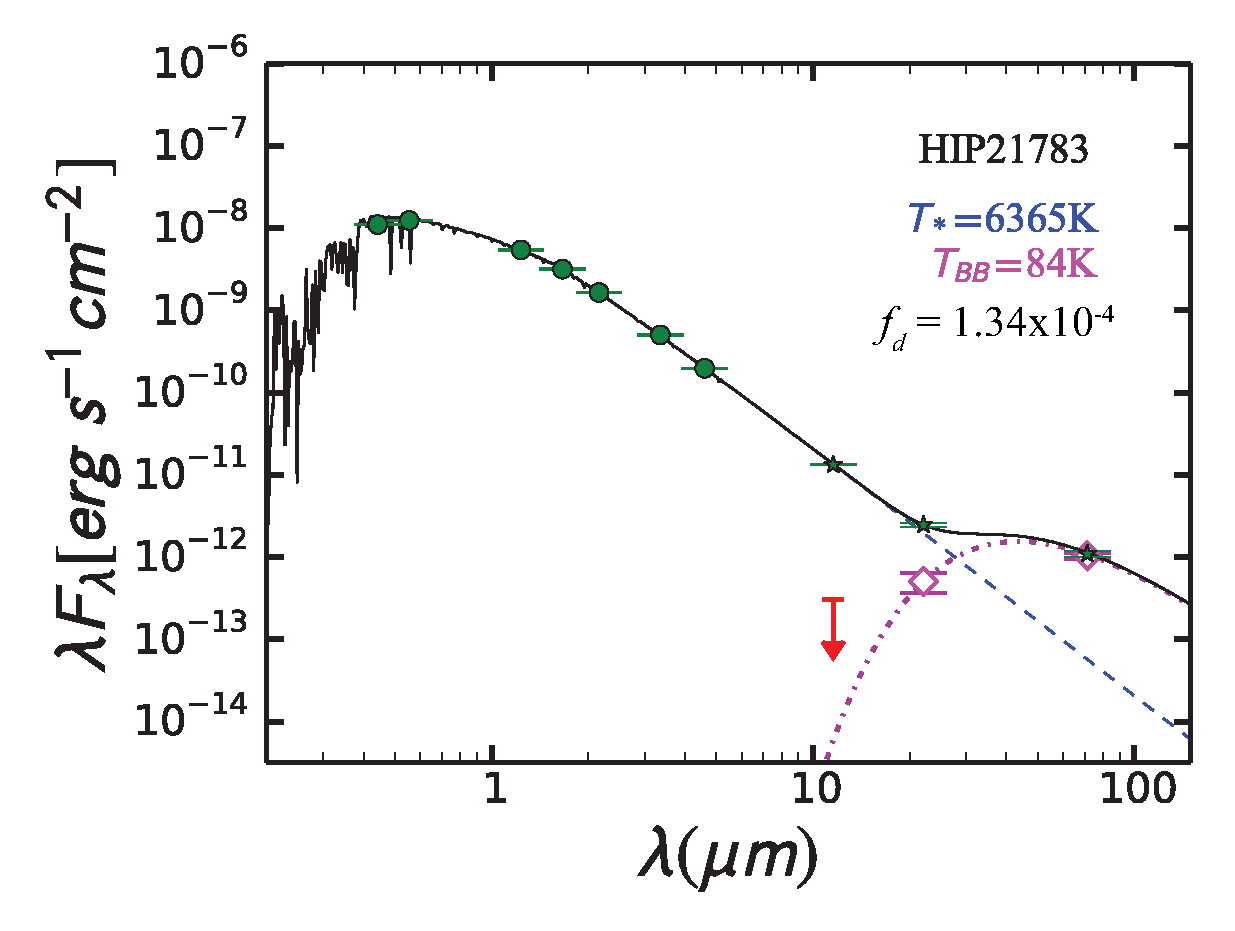
\includegraphics[scale=0.4]{Ch4/HIP21783} &
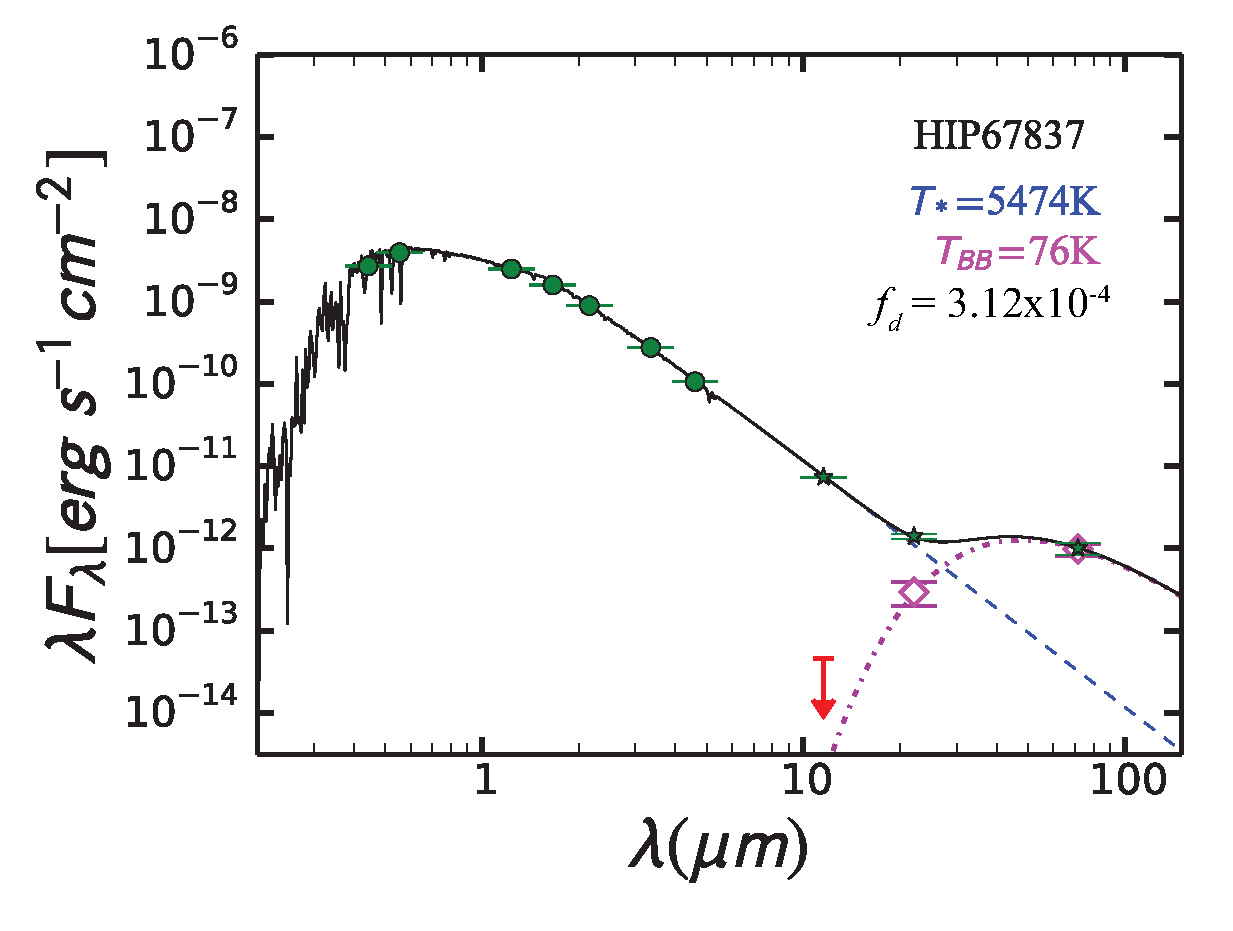
\includegraphics[scale=0.4]{Ch4/HIP67837} \\
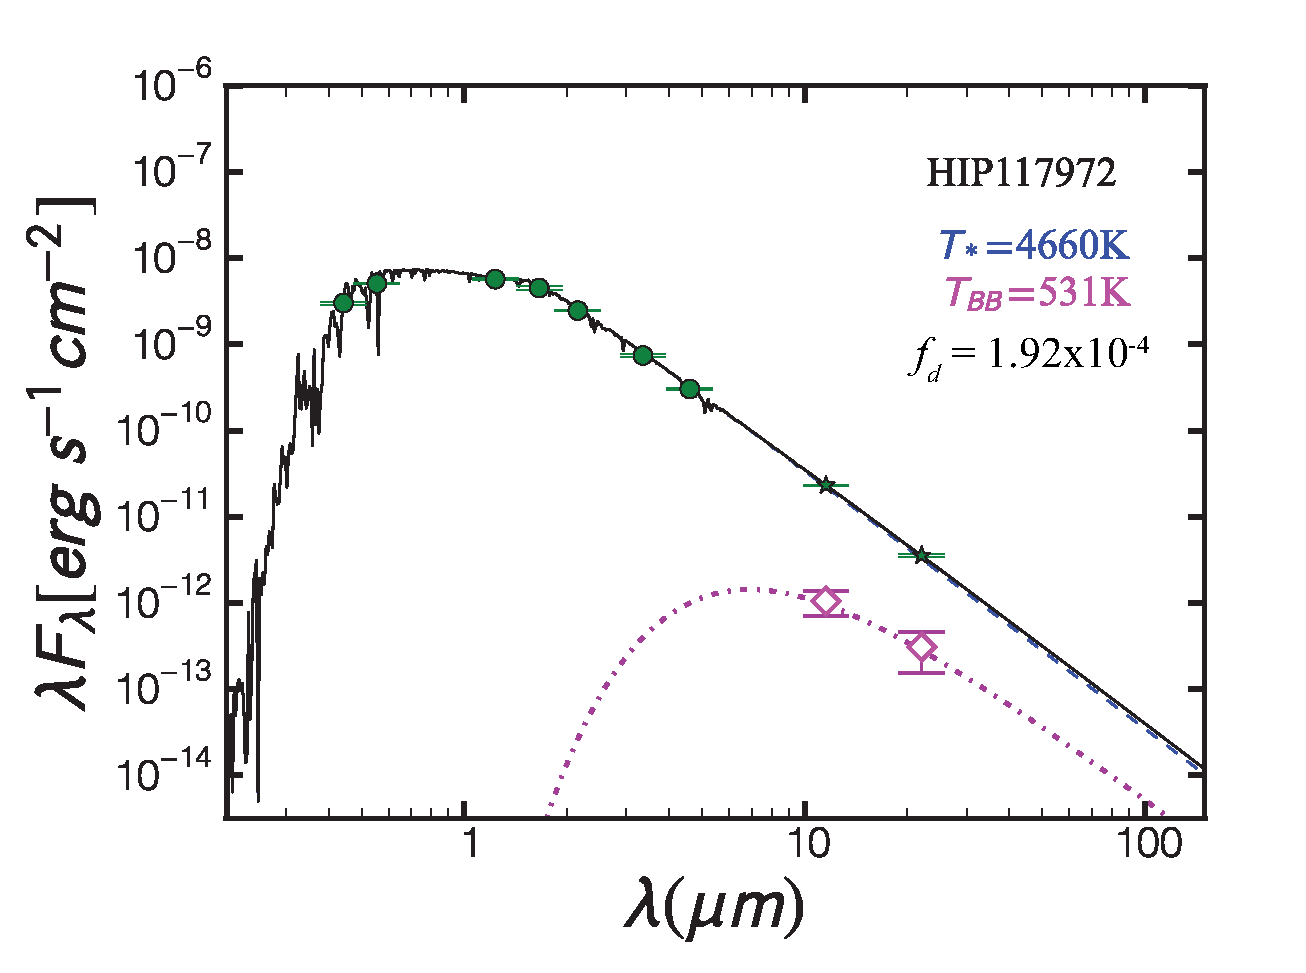
\includegraphics[scale=0.4]{Ch4/HIP117972} &
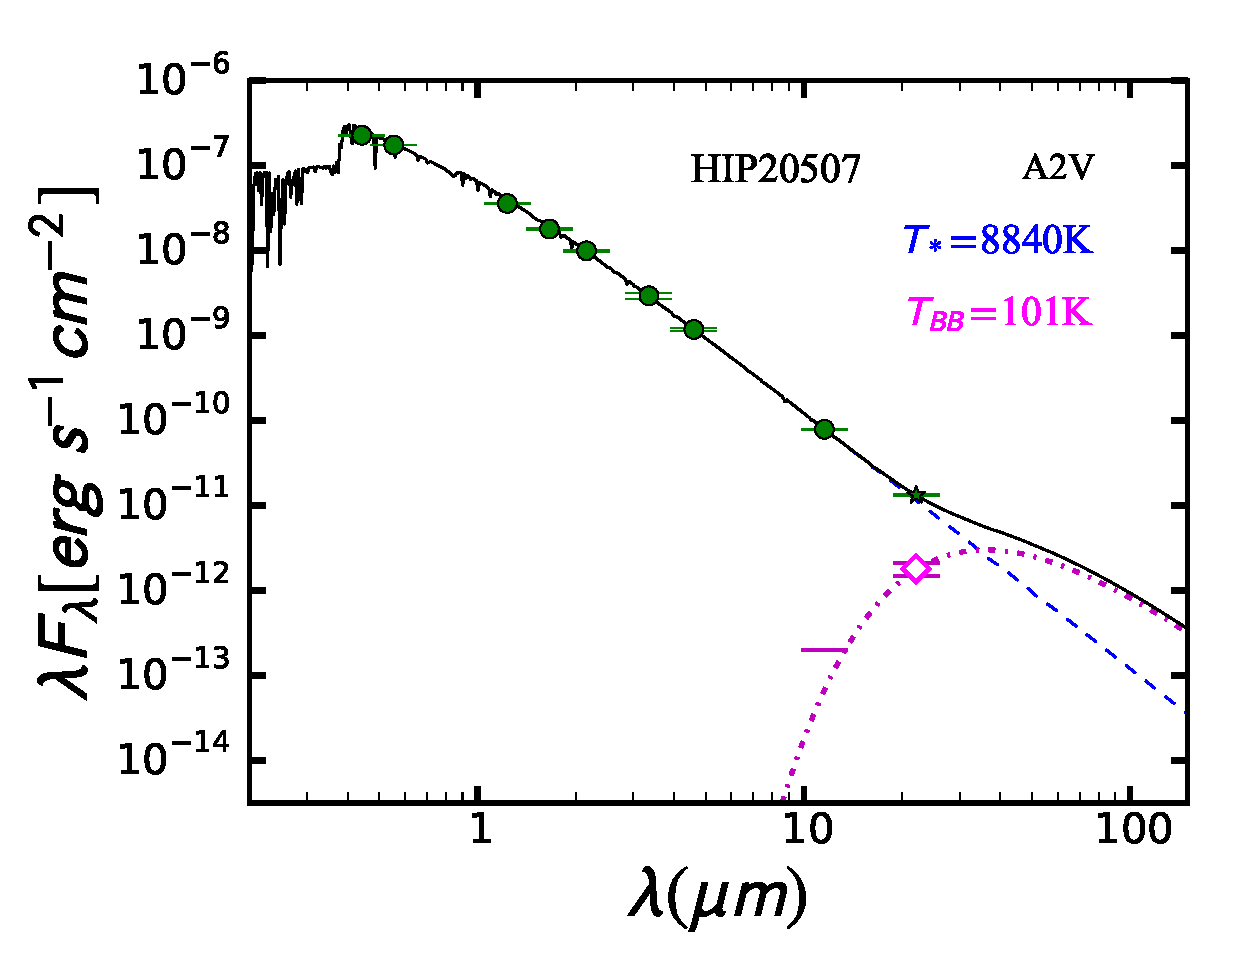
\includegraphics[scale=0.4]{Ch4/HIP20507}
\end{tabular}
\caption{SEDs of newly detected excesses from this study. In each plot, the blue dashed lines correspond to the fitted NextGen photosphere models using photometry indicated by the green circles. The photospheric fit was performed using the BVJHKs photometry from the Hipparcos Catalogue and 2MASS Point Source Catalog, as well as the $W1$ and $W2$ fluxes.  After fitting, the photosphere was scaled to the weighted average of the $W1$ and $W2$ fluxes. The $W1$ and $W2$ photometry were corrected using saturation correction trends derived in \p14. $W3$ and $W4$ All-Sky photometry are green stars at 12 and 22\micron\ in each plot. We fit blackbody curves (magenta dashed-dot curves) to excess fluxes (open magenta diamonds) and 3$\sigma$ upper limits (red arrows) red-ward of $W3$. The combined photosphere and excess emission for each star is plotted as solid black line. HIP~21783 and HIP~67837 are new $W4$ excesses we identified from the significance of their $W2-W4$ and $W3-W4$ color, respectively. We also use archival Spitzer/MIPS 70\micron\ and Herschel/PACS 70\micron\ fluxes to further constrain the dust temperature fits for HIP~21783 and HIP~67837, respectively. The Spitzer and Herschel fluxes were obtained as described in Section~\ref{sec:newdisk_archival}. In addition, HIP~117972 is a new $W3$-only excess which we identified from the significance of its $W1-W3$ color, while HIP~20507 is a new weighted-$W4$ excess.}
\label{fig:SEDs}
\end{figure}
